%Version 3.1 December 2024
% See section 11 of the User Manual for version history
%
%%%%%%%%%%%%%%%%%%%%%%%%%%%%%%%%%%%%%%%%%%%%%%%%%%%%%%%%%%%%%%%%%%%%%%
%%                                                                 %%
%% Please do not use \input{...} to include other tex files.       %%
%% Submit your LaTeX manuscript as one .tex document.              %%
%%                                                                 %%
%% All additional figures and files should be attached             %%
%% separately and not embedded in the \TeX\ document itself.       %%
%%                                                                 %%
%%%%%%%%%%%%%%%%%%%%%%%%%%%%%%%%%%%%%%%%%%%%%%%%%%%%%%%%%%%%%%%%%%%%%

%%\documentclass[referee,sn-basic]{sn-jnl}% referee option is meant for double line spacing

%%=======================================================%%
%% to print line numbers in the margin use lineno option %%
%%=======================================================%%

%%\documentclass[lineno,pdflatex,sn-basic]{sn-jnl}% Basic Springer Nature Reference Style/Chemistry Reference Style

%%=========================================================================================%%
%% the documentclass is set to pdflatex as default. You can delete it if not appropriate.  %%
%%=========================================================================================%%

%%\documentclass[sn-basic]{sn-jnl}% Basic Springer Nature Reference Style/Chemistry Reference Style

%%Note: the following reference styles support Namedate and Numbered referencing. By default the style follows the most common style. To switch between the options you can add or remove “Numbered” in the optional parenthesis. 
%%The option is available for: sn-basic.bst, sn-chicago.bst%  
 
%%\documentclass[pdflatex,sn-nature]{sn-jnl}% Style for submissions to Nature Portfolio journals
%%\documentclass[pdflatex,sn-basic]{sn-jnl}% Basic Springer Nature Reference Style/Chemistry Reference Style
%\documentclass[pdflatex,sn-mathphys-num]{sn-jnl}% Math and Physical Sciences Numbered Reference Style
%%\documentclass[pdflatex,sn-mathphys-ay]{sn-jnl}% Math and Physical Sciences Author Year Reference Style
%%\documentclass[pdflatex,sn-aps]{sn-jnl}% American Physical Society (APS) Reference Style
%%\documentclass[pdflatex,sn-vancouver-num]{sn-jnl}% Vancouver Numbered Reference Style
%%\documentclass[pdflatex,sn-vancouver-ay]{sn-jnl}% Vancouver Author Year Reference Style
%%\documentclass[pdflatex,sn-apa]{sn-jnl}% APA Reference Style
%%\documentclass[pdflatex,sn-chicago]{sn-jnl}% Chicago-based Humanities Reference Style

%%%% Standard Packages
%%<additional latex packages if required can be included here>
%\usepackage[utf8]{inputenc}

%\usepackage{graphicx}%
%\usepackage{multirow}%
%\usepackage{amsmath,amssymb,amsfonts}%
%\usepackage{amsthm}%
%\usepackage{mathrsfs}%
%\usepackage[title]{appendix}%
%\usepackage{xcolor}%
%\usepackage{textcomp}%
%\usepackage{manyfoot}%
%\usepackage{newunicodechar}
%\newunicodechar{₀}{$_0$}
%\newunicodechar{₁}{$_1$}
%\newunicodechar{₂}{$_2$}
%\newunicodechar{₃}{$_3$}
%\newunicodechar{₄}{$_4$}
%\newunicodechar{₅}{$_5$}
%\newunicodechar{₆}{$_6$}
%\newunicodechar{₇}{$_7$}
%\newunicodechar{₈}{$_8$}
%\newunicodechar{₉}{$_9$}
%\usepackage{newunicodechar}
%\newunicodechar{ᵗ}{\textsuperscript{t}}
%\newunicodechar{ʰ}{\textsuperscript{h}}
%\usepackage{newunicodechar}
%\newunicodechar{₀}{$_0$}
%\usepackage{textgreek}
%\usepackage{newunicodechar}
%\newunicodechar{−}{-}
%\usepackage{booktabs}%
%\usepackage{algorithm}%
%\usepackage{algorithmicx}%
%\usepackage{algpseudocode}%
%\usepackage{listings}%
%%%%

%%%%%=============================================================================%%%%
%%%%  Remarks: This template is provided to aid authors with the preparation
%%%%  of original research articles intended for submission to journals published 
%%%%  by Springer Nature. The guidance has been prepared in partnership with 
%%%%  production teams to conform to Springer Nature technical requirements. 
%%%%  Editorial and presentation requirements differ among journal portfolios and 
%%%%  research disciplines. You may find sections in this template are irrelevant 
%%%%  to your work and are empowered to omit any such section if allowed by the 
%%%%  journal you intend to submit to. The submission guidelines and policies 
%%%%  of the journal take precedence. A detailed User Manual is available in the 
%%%%  template package for technical guidance.
%%%%%=============================================================================%%%%

%% as per the requirement new theorem styles can be included as shown below
%\theoremstyle{thmstyleone}%
%\newtheorem{theorem}{Theorem}%  meant for continuous numbers
%%\newtheorem{theorem}{Theorem}[section]% meant for sectionwise numbers
%% optional argument [theorem] produces theorem numbering sequence instead of independent numbers for Proposition
%\newtheorem{proposition}[theorem]{Proposition}% 
%%\newtheorem{proposition}{Proposition}% to get separate numbers for theorem and proposition etc.

%\theoremstyle{thmstyletwo}%
%\newtheorem{example}{Example}%
%\newtheorem{remark}{Remark}%

%\theoremstyle{thmstylethree}%
%\newtheorem{definition}{Definition}%

%\raggedbottom
%%\unnumbered% uncomment this for unnumbered level heads

%\begin{document}

%\title[Article Title]{Article Title}

%%=============================================================%%
%% GivenName	-> \fnm{Joergen W.}
%% Particle	-> \spfx{van der} -> surname prefix
%% FamilyName	-> \sur{Ploeg}
%% Suffix	-> \sfx{IV}
%% \author*[1,2]{\fnm{Joergen W.} \spfx{van der} \sur{Ploeg} 
%%  \sfx{IV}}\email{iauthor@gmail.com}
%%=============================================================%%

\documentclass[9pt,twocolumn,twoside]{rilabRxiv}
% Use the documentclass option 'lineno' to view line numbers
\setlength{\marginparwidth}{2cm}
\usepackage[textsize=tiny,colorinlistoftodos]{todonotes}
\definecolor{cornflowerblue}{rgb}{0.39, 0.58, 0.93}

% Custom macros from main_20251203.tex
\usepackage{xspace}
\usepackage{booktabs}
\usepackage{multirow}
\usepackage{pdfpages}

% Set supplement numbers to S and start counting newly
\newcommand{\beginsupplement}{%
  \setcounter{table}{0}
  \renewcommand{\thetable}{S\arabic{table}}%
  \setcounter{figure}{0}
  \renewcommand{\thefigure}{S\arabic{figure}}%
}

% Custom commands from source
\newcommand{\mex}{\textit{mexicana}\xspace}
\newcommand{\invfour}{\textit{Inv4m}\xspace}
\newcommand{\fdrgt} {$\textrm{\textit{FDR}} > 0.05$}
\newcommand{\fdreq} {$\textrm{\textit{FDR}} = 0.05$}
\newcommand{\fdrls} {$\textrm{\textit{FDR}} < 0.05$}
\newcommand{\parv}{\textit{parviglumis}\xspace}
\newcommand{\jmjii}{\textit{jmj2}\xspace}
\newcommand{\jmjiv}{\textit{jmj4}\xspace}
\newcommand{\jmjvi}{\textit{jmj6}\xspace}
\newcommand{\jmjix}{\textit{jmj9}\xspace}
\newcommand{\arabidopis}{\textit{Arabidopsis}\xspace}

\usepackage[hyperfigures=false]{hyperref}

\newcolumntype{b}{X}
\newcolumntype{s}{>{\hsize=.5\hsize}X}
\title{Integrative quantitative genetics implicates aspartate-family amino acid metabolism and protein turnover in grain nitrogen accumulation and remobilization in maize}

%\title{Introgression of the teosinte \mex chromosomal inversion \textit{Inv4m} modulates maize flowering time, plant height, and growth regulation gene networks in a temperate genetic background}

% Teosinte Inv4m Inversion Modulates Maize Growth and Flowering via Gene Network Rewiring


\author[$1$]{Nirwan Tandukar}
\author[$2$]{Sarah Fitzsimmons}
\author[$3$]{Sherry Flint Garcia}
\author[$4$]{Ruthie Angelovici}
\author[$5$]{Rubén Rellán-Álvarez}

\affil[$1$]{Department of Molecular and Structural Biochemistry, N.C. Plant Sciences Initiative, Genetics and Genomics Program, North Carolina State University, Raleigh, NC, USA}
\affil[$2$]{Division of Biological Sciences, University of Missouri, Columbia, MO 65211, USA}
\affil[$3$]{Division of Biological Sciences, Interdisciplinary Plant Group, Christopher S. Bond Life Sciences Center, University of Missouri, Columbia, MO 65211, USA}
\affil[$4$]{USDA-ARS Plant Genetics Research Unit, Columbia, MO 65211, USA}
\affil[$5$]{Department of Molecular and Structural Biochemistry, N.C. Plant Sciences Initiative, North Carolina State University, Raleigh, NC, USA}



\keywords{Maize natural variation, nitrogen efficiency, maize kernel aminoacids}

\runningtitle{Maize grain nitrogen natural variation}
%% last names of both authors if there are two authors;
% \runningauthor{FirstAuthorLastname and SecondAuthorLastname}
%% last name of the first author followed by et al, if more than two authors.
\runningauthor{Tandukar \textit{et al.}}


%%% Abstract %%%%%%%%%%%%%%%%%%
\begin{abstract}
Grain nitrogen accumulation in maize integrates inorganic N uptake, assimilation into aspartate- and glutamate-family amino acids, protein synthesis, and remobilization from vegetative tissues. 
The genetic architecture coordinating these processes remains incompletely resolved. 
Here we combine quantitative genetic analyses across four complementary populations to dissect grain N variation in maize.
Protein-bound and free amino acid profiling of the Goodman–Buckler association panel identified asparagine and proline as the dominant amino acids in mature grain. 
Genome-wide association studies of total protein, a proxy for grain nitrogen content, and 110 free amino acid traits identified candidate loci enriched for aspartate-family metabolism and nitrogen assimilation, with biparental QTL mapping in a B64 × CML14 population further refining loci controlling grain asparagine accumulation. 
An environmental GWAS across 3,511 georeferenced landraces (Romero Navarro et al.) recovered soil-nitrogen–associated candidates including an omega-amidase/NIT2-like CN hydrolase (Zm00001eb005710) and an aspartate kinase (Zm00001eb220040), linking environmental N availability to aspartate–asparagine–glutamine metabolism. 
In parallel, we used skim sequencing and free amino acid profiling of the Indian Chief and Jarvis open-pollinated populations across 14 cycles of reciprocal recurrent selection to test how selection on grain yield has reshaped N allocation. 
Indian Chief Cycle 14 showed a strong shift toward proline-dominated free amino acid pools with reduced aspartate and glutamate fractions, while Jarvis showed an opposing, underpowered trend. 
Concordant FST, Tajima's D, and nucleotide-diversity scans identified candidate regions enriched for autophagy, ubiquitin–proteasome components, and proteases — including the autophagy-related gene Zm00001eb372060, the only candidate jointly supported by selection scans and the proline GWAS. 
Together, these results highlight aspartate-family metabolism and protein turnover as recurring genetic axes underlying both natural variation and selection-driven divergence in maize grain nitrogen.
\end{abstract}
%%%%%%%%%%%%%%%%%%%%%%%%%%

\setboolean{displaycopyright}{true}

\begin{document}

\maketitle
\thispagestyle{firststyle}
\correspondingauthoraffiliation{
Department of Molecular and Structural Biochemistry, N.C. Plant Sciences Initiative, North Carolina State University, Raleigh, NC, USA. 
E-mail: frodrig4@ncsu.edu, rrellan@ncsu.edu}
\vspace{-11pt}%

\setboolean{displaylineno}{true}
\ifthenelse{\boolean{displaylineno}}{\linenumbers}{}

\section{Introduction}

\lettrine[lines=2]{\color{color2}I}{n} most modern varieties of maize, inorganic nitrogen is taken up by the roots as nitrate or ammonium. Nitrate is reduced into nitrite by nitrate reductases and can then be stored in root tissue. Alternatively, nitrite and ammonium can be assimilated into organic forms, such as amino acids. They can be freely transported through xylem and phloem, with intracellular transport being facilitated by amino acid transporters or permeases. Storage of nitrogen stores typically occurs in sink tissues, such as the kernels, through free amino acid (FAA) pools or amino acids bound in proteins, or PBAAs.
Among these, aspartate (Asp) and asparagine (Asn), and to a lesser extent, glutamate (Glu) and glutamine (Gln), play important roles in nitrogen assimilation and storage. Asp and Glu are key intermediates in the incorporation of inorganic nitrogen into organic molecules, while Asn and Gln serve as major nitrogen transport and storage compounds due to their high nitrogen-to-carbon ratios and stability. As nitrogen demand increases, these amino acids are degraded to release assimilated nitrogen for metabolic use. In nitrogen-rich environments, elevated levels of free Asn, Asp, Gln, and Glu, as well as increased protein accumulation, have been observed.


Quantitative genetic studies have proven to be an effective way to elucidate the genetic architecture of complex traits, such as grain nitrogen. Genome-wide association studies (GWAS) are a powerful tool used to identify SNPs associated with phenotypic variation. However, traditional GWAS often yields a large number of associations, many of which may not be biologically meaningful. To address this, it is best to employ one or more additional quantitative approaches to further clarify results. In environmentally dependent traits, environmental GWAS (envGWAS), which integrates environmental covariates into the association analysis to identify SNPs whose effects vary across environmental gradients, is a valuable complementary method. This approach helps reduce spurious associations and enhances the detection of loci involved in genotype-by-environment interactions, providing a more nuanced understanding of trait architecture. To maximize the power and resolution of these analyses, we leveraged two distinct populations: the Goodman-Buckler Association panel, a diverse inbred panel for GWAS which captures broad allelic variation, and a biparental population derived from two landraces, Indian Chief and Jarvis, that are adapted to contrasting soil nitrogen conditions for envGWAS, enabling the detection of environment-specific genetic effects.


\section{Results}\label{results}


\subsection{Amino acid profiling identifies asparagine and proline as the predominant amino acids} 

\paragraph{Total Protein and Nitrogen Proxy GWAS}
Total protein can reasonably be calculated from the sum of each PBAA. Our GWAS of total PBAA yielded 16 significant SNPs that contained 501 unique candidate genes within a 200kb region. The majority of these associations were detected using the BLINK and FarmCPU models, with only two SNPs identified by MLMM. Notably, one SNP (7-5322774) was consistently identified across all three models. Though grain protein accounts for a large proportion of the nitrogen found in the grain, it may not accurately represent the levels of nitrogen present due to variances in amino acid composition and levels of free amino acids. For this reason we opted to calculate a proxy nitrogen content that takes these factors into account. GWAS of proxy nitrogen also yielded 16 significant SNPs, though only four overlapped with those identified for total protein. These proxy nitrogen SNPs were associated with 489 candidate genes, 173 of which were also found in the total protein results. As with total protein, most associations were identified using BLINK and FarmCPU. One SNP (1-80777231) was identified by all three models for proxy nitrogen and was also detected in both BLINK and MLMM for total protein. These results suggest that while total protein and proxy nitrogen share some genetic architecture, they also capture distinct aspects of nitrogen-related variation. 



\paragraph{Free Amino Acid GWAS}
In addition to the total PBAA and proxy nitrogen traits, we evaluated 110 additional traits related to free amino acid (FAA) accumulation in maize grain. These included the absolute concentrations of all 20 proteinogenic amino acids, their relative abundances (as proportions of total FAAs), and a set of biochemical ratios comparing individual amino acids and their metabolic families. Across the 112 traits, we identified a total of XX,XXX significant SNPs using four GWAS models: BLINK, FarmCPU, MLM, and MLMM. After applying FDR correction, XX,XXX SNPs remained significant, corresponding to XX,XXX candidate genes. To better understand the genetic basis of nitrogen accumulation in maize grain, we focused on traits related to asparagine (Asn), aspartate (Asp), glutamine (Gln), and glutamate (Glu), given their central roles in nitrogen assimilation and transport. In addition to their absolute and relative abundances, we analyzed 11 biochemical ratios involving the glutamate and aspartate amino acid families. Across these 19 traits, we detected 649 significant SNPs: 478 from FarmCPU, 220 from BLINK, 21 from MLMM, and 16 from MLM. Within a 200 kb window of these SNPs, we identified 14,639 candidate genes.


\subsection{B64 × CML14 biparental mapping identifies candidate loci for grain asparagine accumulation}



\subsection{Soil nitrogen enviornment GWAS highlights aspartate-family and asparagine metabolism in maize landrace adaptation}

We next asked whether natural variation in maize landraces could provide insight into the genetic basis of amino acid variation, including asparagine. To address this, we integrated the Romero Navarro \textit{et al.} maize landrace panel with total soil nitrogen for each accession. The sampled landraces span Mexico, Central America, and South America, and they capture broad variation in soil nitrogen availability (Fig.~\ref{fig:soilN_gwas}A). This provides a framework to test natural genetic variation associated with soil nitrogen gradients.

We performed GWAS using a mixed linear model with three genotype principal components as covariates, and also applied MLM, MLMM, BLINK, and FarmCPU, summarizing the strongest signals across the models (Fig.~\ref{fig:soilN_gwas}B). The GWAS identified multiple loci exceeding the Bonferroni significance thresholds (Supplementary Fig.~\ref{fig:supp_soiln_qq_venn} A). Model overlap analysis showed that BLINK and FarmCPU yielded most of high-confidence signals, with 79 SNPs shared between them and six SNPs shared across all four models (Supplementary Fig.~\ref{fig:supp_soiln_qq_venn} B).


\begin{figure*}[ht!]
\centering
    \centering
    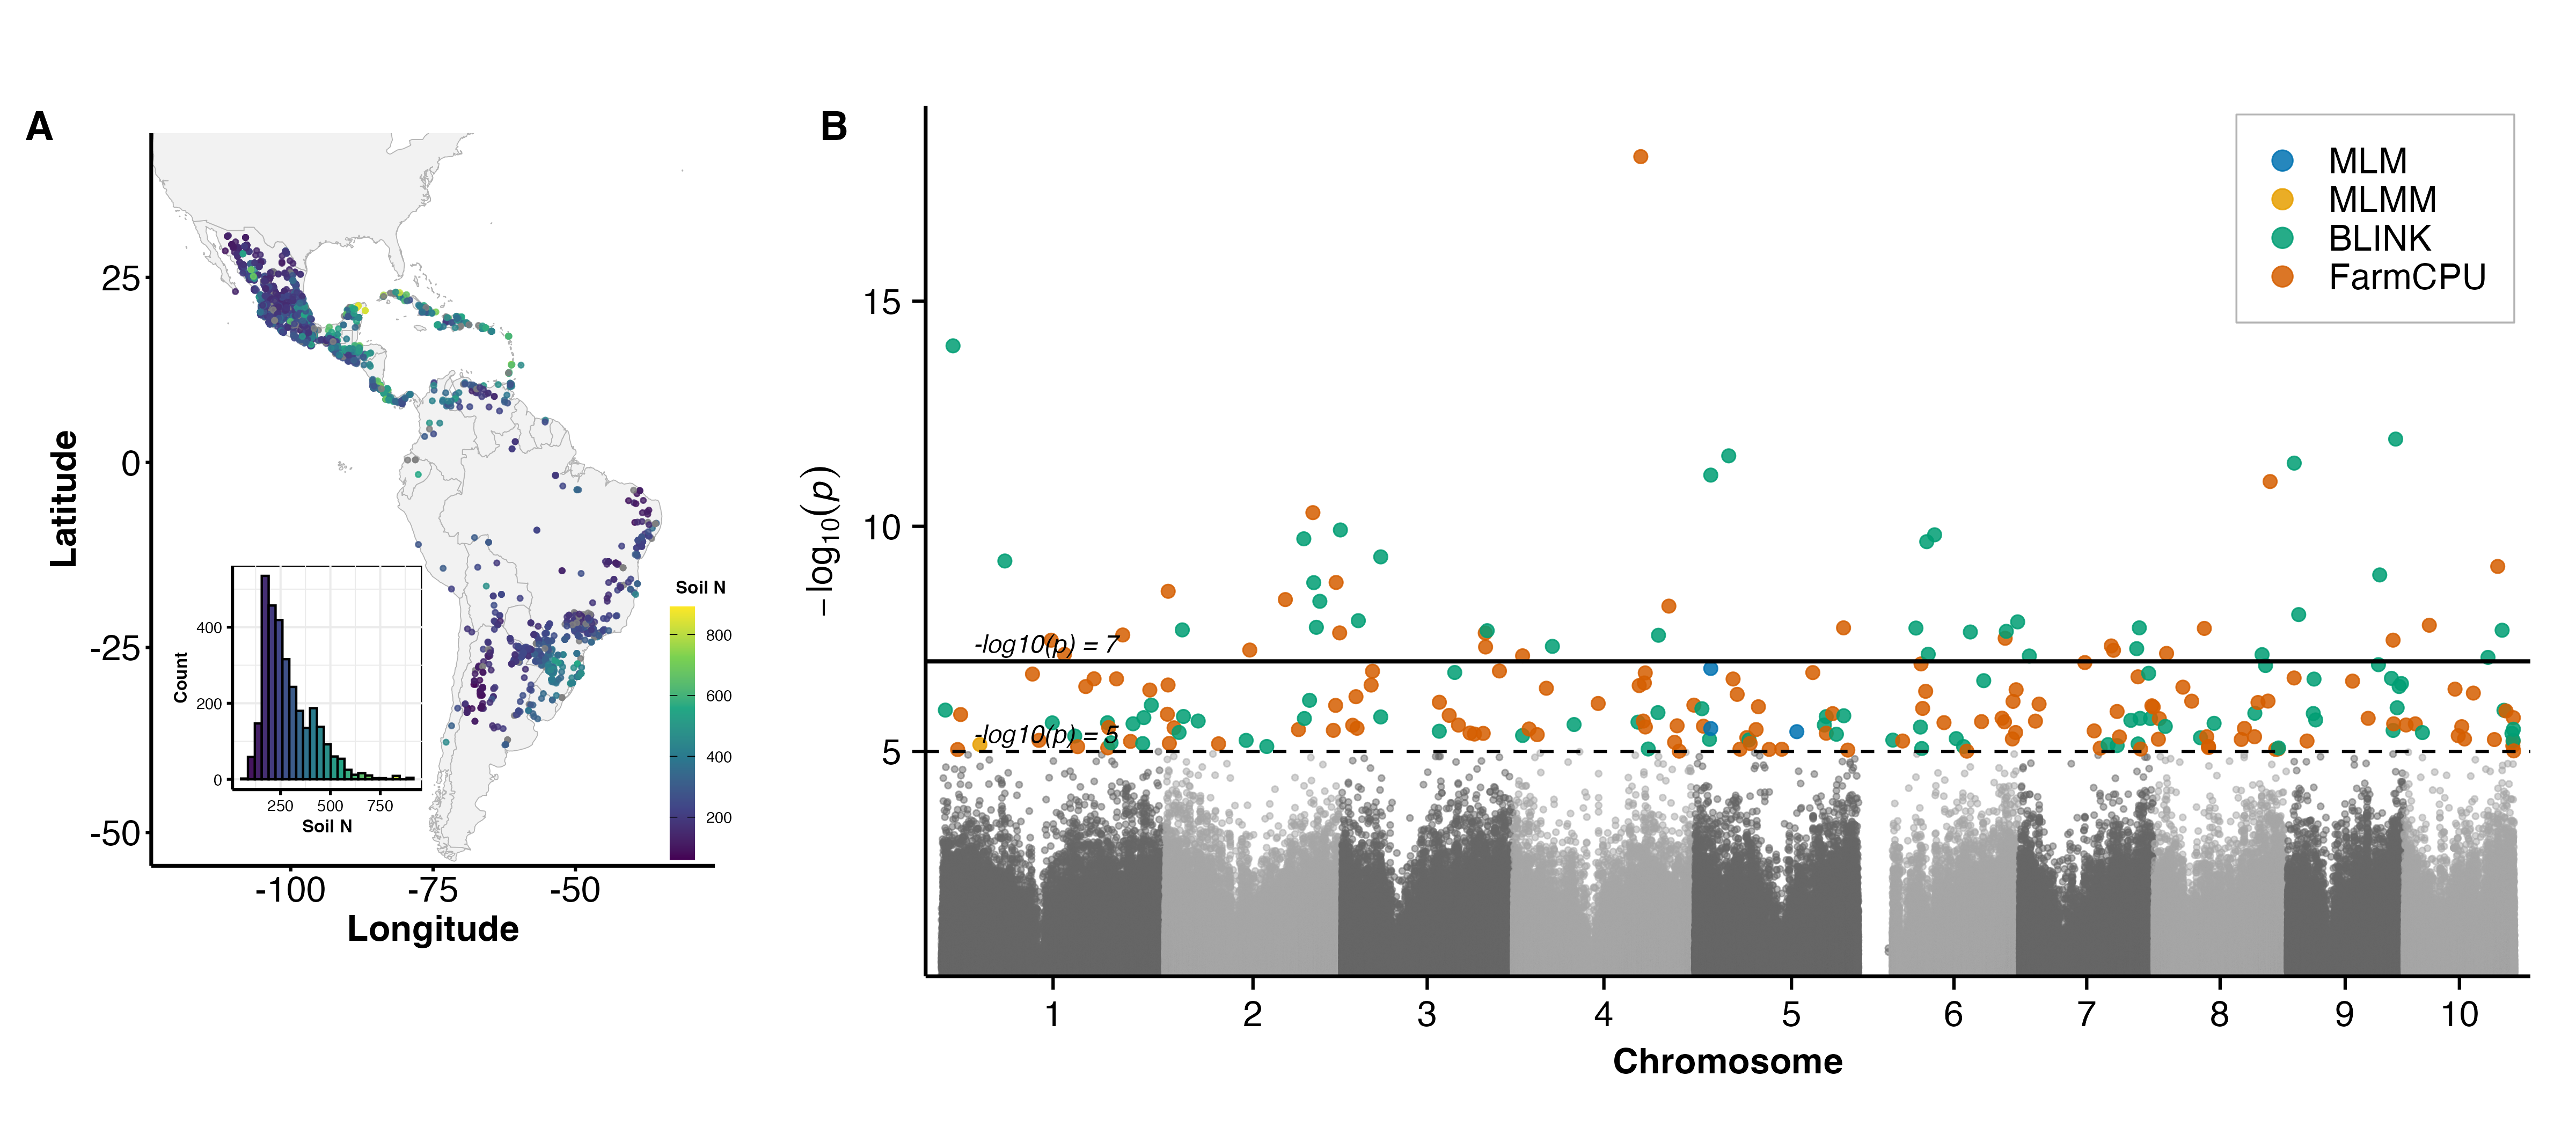
\includegraphics[width=\linewidth]{Figs/main/Fig1.png}
    \caption{Geographic distribution of soil nitrogen and genome-wide association results for soil N. \textbf{A}, Sampling locations across the Americas colored by soil N, with an inset histogram showing the soil N distribution across accessions. \textbf{B}, Manhattan plot of soil N GWAS results across chromosomes. Colored points indicate loci identified by the MLM, MLMM, BLINK, and FarmCPU models. Horizontal lines indicate suggestive and more stringent significance thresholds.}
    \label{fig:soilN_gwas}
\end{figure*}


Two candidates are notable because their functions link soil nitrogen variation to amino acid metabolism. The top candidate, \textit{Zm00001eb005710}, encodes a CN hydrolase domain–containing protein. It shows a strong association with soil N ($-\log\_{10}(P) = 14.01$) and is annotated with omega-amidase/NIT2-like activity, hydrolase activity on carbon–nitrogen bonds, and roles in oxaloacetate, asparagine, and glutamine metabolism. A second candidate, \textit{Zm00001eb220040}, encodes a protein with an aspartate/glutamate/uridylate kinase domain and is associated with soil N at $-\log_{10}(P) = 11.14$. Its Gene Ontology annotations include aspartate kinase activity, amino acid biosynthesis, and threonine biosynthesis. Since aspartate kinase catalyzes an early committed step in the aspartate-family amino acid pathway, this locus is a plausible mediator of soil N effects on downstream amino acid biosynthesis (ref).

Together, these results highlight \textit{Zm00001eb220040} and \textit{Zm00001eb005710} as candidates related to nitrogen-metabolism involved in aspartate, asparagine, and glutamine metabolism. These inferences are based on annotations and GO terms rather than direct experiments and should be viewed cautiously. Nonetheless, the alignment of soil N GWAS signals with amino acid metabolism–related annotations supports a mechanistic link between environmental nitrogen availability and grain nitrogen-associated metabolic pathways.



\subsection{Free amino acid analysis in Indian Chief and Jarvis implicate protein turnover in population-specific N allocation}

To evaluate selection-associated variation in nitrogen accumulation and partitioning, we utilized the Indian Chief and Jarvis maize populations.  These populations derive from long-term recurrent selection experiments in which Jarvis Golden Prolific and Indian Chief served as open-pollinated base populations, and selection for 14 cycles targeted grain weight per plant as the sole direct criterion \citep{Moll1994}. Previous phenotypic work showed that reciprocal recurrent selection altered nitrogen allocation differently in Jarvis and Indian Chief. At nonlimiting N supply, Jarvis, after 14 cycles of reciprocal recurrent selection, accumulated greater grain N and showed greater post-anthesis loss of N from stover relative to the original Jarvis population. In contrast, Indian Chief, after 14 cycles of reciprocal recurrent selection, showed increased post-anthesis stover biomass but had lower grain weight, lower post-anthesis loss of N from stover, and no significant increase in grain N relative to the original Indian Chief population \citep{Moll1994}.

We analyzed selected FAA abundance and composition metrics in the IC and J populations at Cycle~0 and Cycle~14 (Supplementary Fig.~\ref{fig:supp_ic_j_amino_profiles}; Supplementary Table~\ref{tab:supp_ic_j_amino_profile_stats}). Indian Chief showed significant remodeling of both total FAA abundance and relative FAA composition. Total FAA abundance increased from 7.62 in Cycle~0 to 13.42 in Cycle~14 (Wilcoxon rank-sum $p = 0.0043$; BH-adjusted $p = 0.0194$), indicating expansion of the measured free amino acid pool. Within this expanded pool, proline became more dominant: the proline fraction increased from 0.320 to 0.519 ($p = 0.0157$; BH-adjusted $p = 0.0283$). In contrast, acidic amino acids decreased as fractions of the total FAA pool. Aspartate fraction decreased from 0.115 to 0.075 ($p = 0.0157$; BH-adjusted $p = 0.0283$), and glutamate fraction decreased from 0.140 to 0.062 ($p = 0.0068$; BH-adjusted $p = 0.0203$). Thus, Indian Chief Cycle~14 showed both increased total FAA abundance and a compositional shift away from Asp/Glu fractions and toward proline enrichment. This shift is relevant because the soil N GWAS identified candidate genes connected to aspartate/asparagine and glutamine metabolism, including an aspartate kinase candidate. Therefore, the FAA data do not simply show proline accumulation; they also show that the relative contribution of Asp and Glu to the FAA pool changed significantly after selection. Together, these results suggest that Indian Chief Cycle~14 underwent broader remodeling of amino acid allocation, with proline enrichment occurring alongside reduced Asp/Glu representation in the total FAA pool.


Jarvis showed a weaker and statistically underpowered pattern because the Cycle~0 group contained only three biological samples. Total FAA abundance was numerically lower in Cycle~14 than in Cycle~0 (9.89 vs.\ 13.41; Wilcoxon rank-sum $p = 0.3583$; BH-adjusted $p = 0.6271$), and the proline fraction also decreased numerically from 0.455 to 0.322 ($p = 0.1846$; BH-adjusted $p = 0.4307$). The N-rich FAA pool showed a similar numerical decrease from 2.35 to 1.80 ($p = 0.1846$; BH-adjusted $p = 0.4307$). In contrast to Indian Chief, the aspartate fraction increased from 0.075 to 0.137 in Cycle~14. This change was nominally significant before multiple-testing correction ($p = 0.0189$), but it was not significant after BH correction ($p = 0.1323$). Glutamate fraction changed only modestly from 0.081 to 0.087 and was not significant ($p = 0.9187$; BH-adjusted $p = 1.0000$). Thus, Jarvis showed a directional but underpowered pattern toward lower total FAA, lower proline fraction, and higher Asp representation in Cycle~14.

Together, the FAA data indicate that selection-associated amino acid remodeling differed between the two populations. Indian Chief showed a strong and statistically supported shift toward proline-dominated FAA composition, with increased total FAA abundance, increased proline fraction, and reduced Asp/Glu fractions in Cycle~14. In Jarvis, the comparison was underpowered, but the direction of change differed from Indian Chief: proline fraction was numerically lower in Cycle~14, whereas Asp fraction was numerically higher. Although these Jarvis trends were not significant after multiple-testing correction, they suggest a possible relative loss of proline representation and increased Asp representation in the Cycle~14 FAA pool, rather than the proline-enrichment pattern observed in Indian Chief.

These FAA measurements were interpreted alongside prior physiological analyses of the same recurrent-selection material, but they should not be treated as direct equivalents of whole-plant N partitioning. Under reciprocal recurrent selection, Jarvis Cycle~14 showed greater grain N accumulation and greater post-anthesis loss of N from stover relative to the original Jarvis population, consistent with stronger transfer of vegetative N toward grain. In contrast, Indian Chief Cycle~14 showed greater post-anthesis stover biomass, reduced post-anthesis loss of N from stover, and no significant increase in grain N relative to the original Indian Chief population \citep{Moll1994}. Thus, the historical physiological data suggest stronger grain-directed N remobilization in Jarvis, whereas our FAA data show clearer accumulation and proline enrichment in Indian Chief Cycle~14.


\subsection{Skim sequencing reveals generation-specific genetic differentiation in Indian Chief and Jarvis}

We also performed skim sequencing on 100 individuals each from the Indian Chief and Jarvis maize populations at Generations~0 and 14. Sample-level sequencing metrics matched expectations for low-coverage skim sequencing (Supplementary Fig.~\ref{fig:seq_sample_level}). Across 379 individuals, mean sequencing depth was 0.73$\times$ (median 0.72$\times$, range 0.32--1.91$\times$). Most samples had 0.5--1.0$\times$ coverage (323/379); 26 were below 0.5$\times$, 29 were between 1.0$\times$ and 1.5$\times$, and one exceeded 1.5$\times$ (Supplementary Fig.~\ref{fig:supp_seq_sample} A,C). Despite the low depth, genotype recovery was high and uniform, with $\sim$59.0 million genotypes called per individual (Supplementary Fig.~\ref{fig:supp_seq_sample} B). Missing data were moderate for skim sequencing, with a median of 102{,}814 missing genotypes per sample, a 95th percentile of 167{,}497, and a maximum of 328{,}163 per individual.

Variant-level summary statistics indicated that the dataset was suitable for population-level genetic analyses. (Supplementary Fig.~\ref{fig:supp_seq_variant}). Per-site sequencing depth was centered near 7$\times$ across retained variants, with an interquartile range of 5–9$\times$ (Supplementary Fig.~\ref{fig:supp_seq_variant} A). The minor allele frequency spectrum was skewed toward low-frequency variants, as expected for segregating breeding populations with substantial standing genetic variation (Supplementary Fig.~\ref{fig:supp_seq_variant} B). Missing genotype counts declined smoothly across samples ranked by missingness, indicating that missing data were not driven by a small subset of problematic individuals (Supplementary Fig.~\ref{fig:supp_seq_variant} C). Transition/transversion ratios were highly consistent across the 10 maize chromosomes (1.74–1.81; genome-wide mean 1.785; Supplementary Fig.~\ref{fig:supp_seq_variant} D). After filtering, 512,667 SNPs were retained, and a linkage-disequilibrium–pruned subset of 57,568 markers was used for population-structure analyses.

Population-structure analyses showed that Indian Chief and Jarvis remained genetically differentiated after 14 generations of selection, while also exhibiting clear generation-associated shifts within each population (Fig.~\ref{fig:fig3}A). Individual ancestry profiles clustered primarily by source population, with little evidence of extensive admixture. Within each population, comparisons between Generation~0 and Generation~14 revealed shifts in inferred ancestry components, consistent with selection-driven allele-frequency changes. Principal component analysis showed similar results. PC1 explained 1.32\% of the variance and primarily separated Indian Chief from Jarvis, whereas PC2 explained 0.83\% and further distinguished Generation~0 from Generation~14 within each population (Fig.~\ref{fig:fig3}B). Thus, long-term selection preserved the ancestral population identities of Indian Chief and Jarvis while generating detectable genome-wide differentiation between ancestral and selected generations.

Shared-SNP summaries provide an additional view of temporal and between-population shifts in allele composition (Fig.~\ref{fig:fig3}C,D). Within populations, Generation~0 individuals shared more SNPs with Generation~14 than vice versa. In Indian Chief, the mean proportion of shared SNPs was ~0.799 for Generation~0 relative to Generation~14, versus 0.371 for Generation~14 relative to Generation~0. Similarly, in Jarvis, the values were ~0.726 and 0.483, respectively (Fig.~\ref{fig:fig3}C). This asymmetry indicates that many ancestral alleles persisted into Generation~14, while selected-generation individuals also carried generation-enriched alleles that were relatively rare in Generation~0.


\begin{figure*}[ht!]
    \centering
    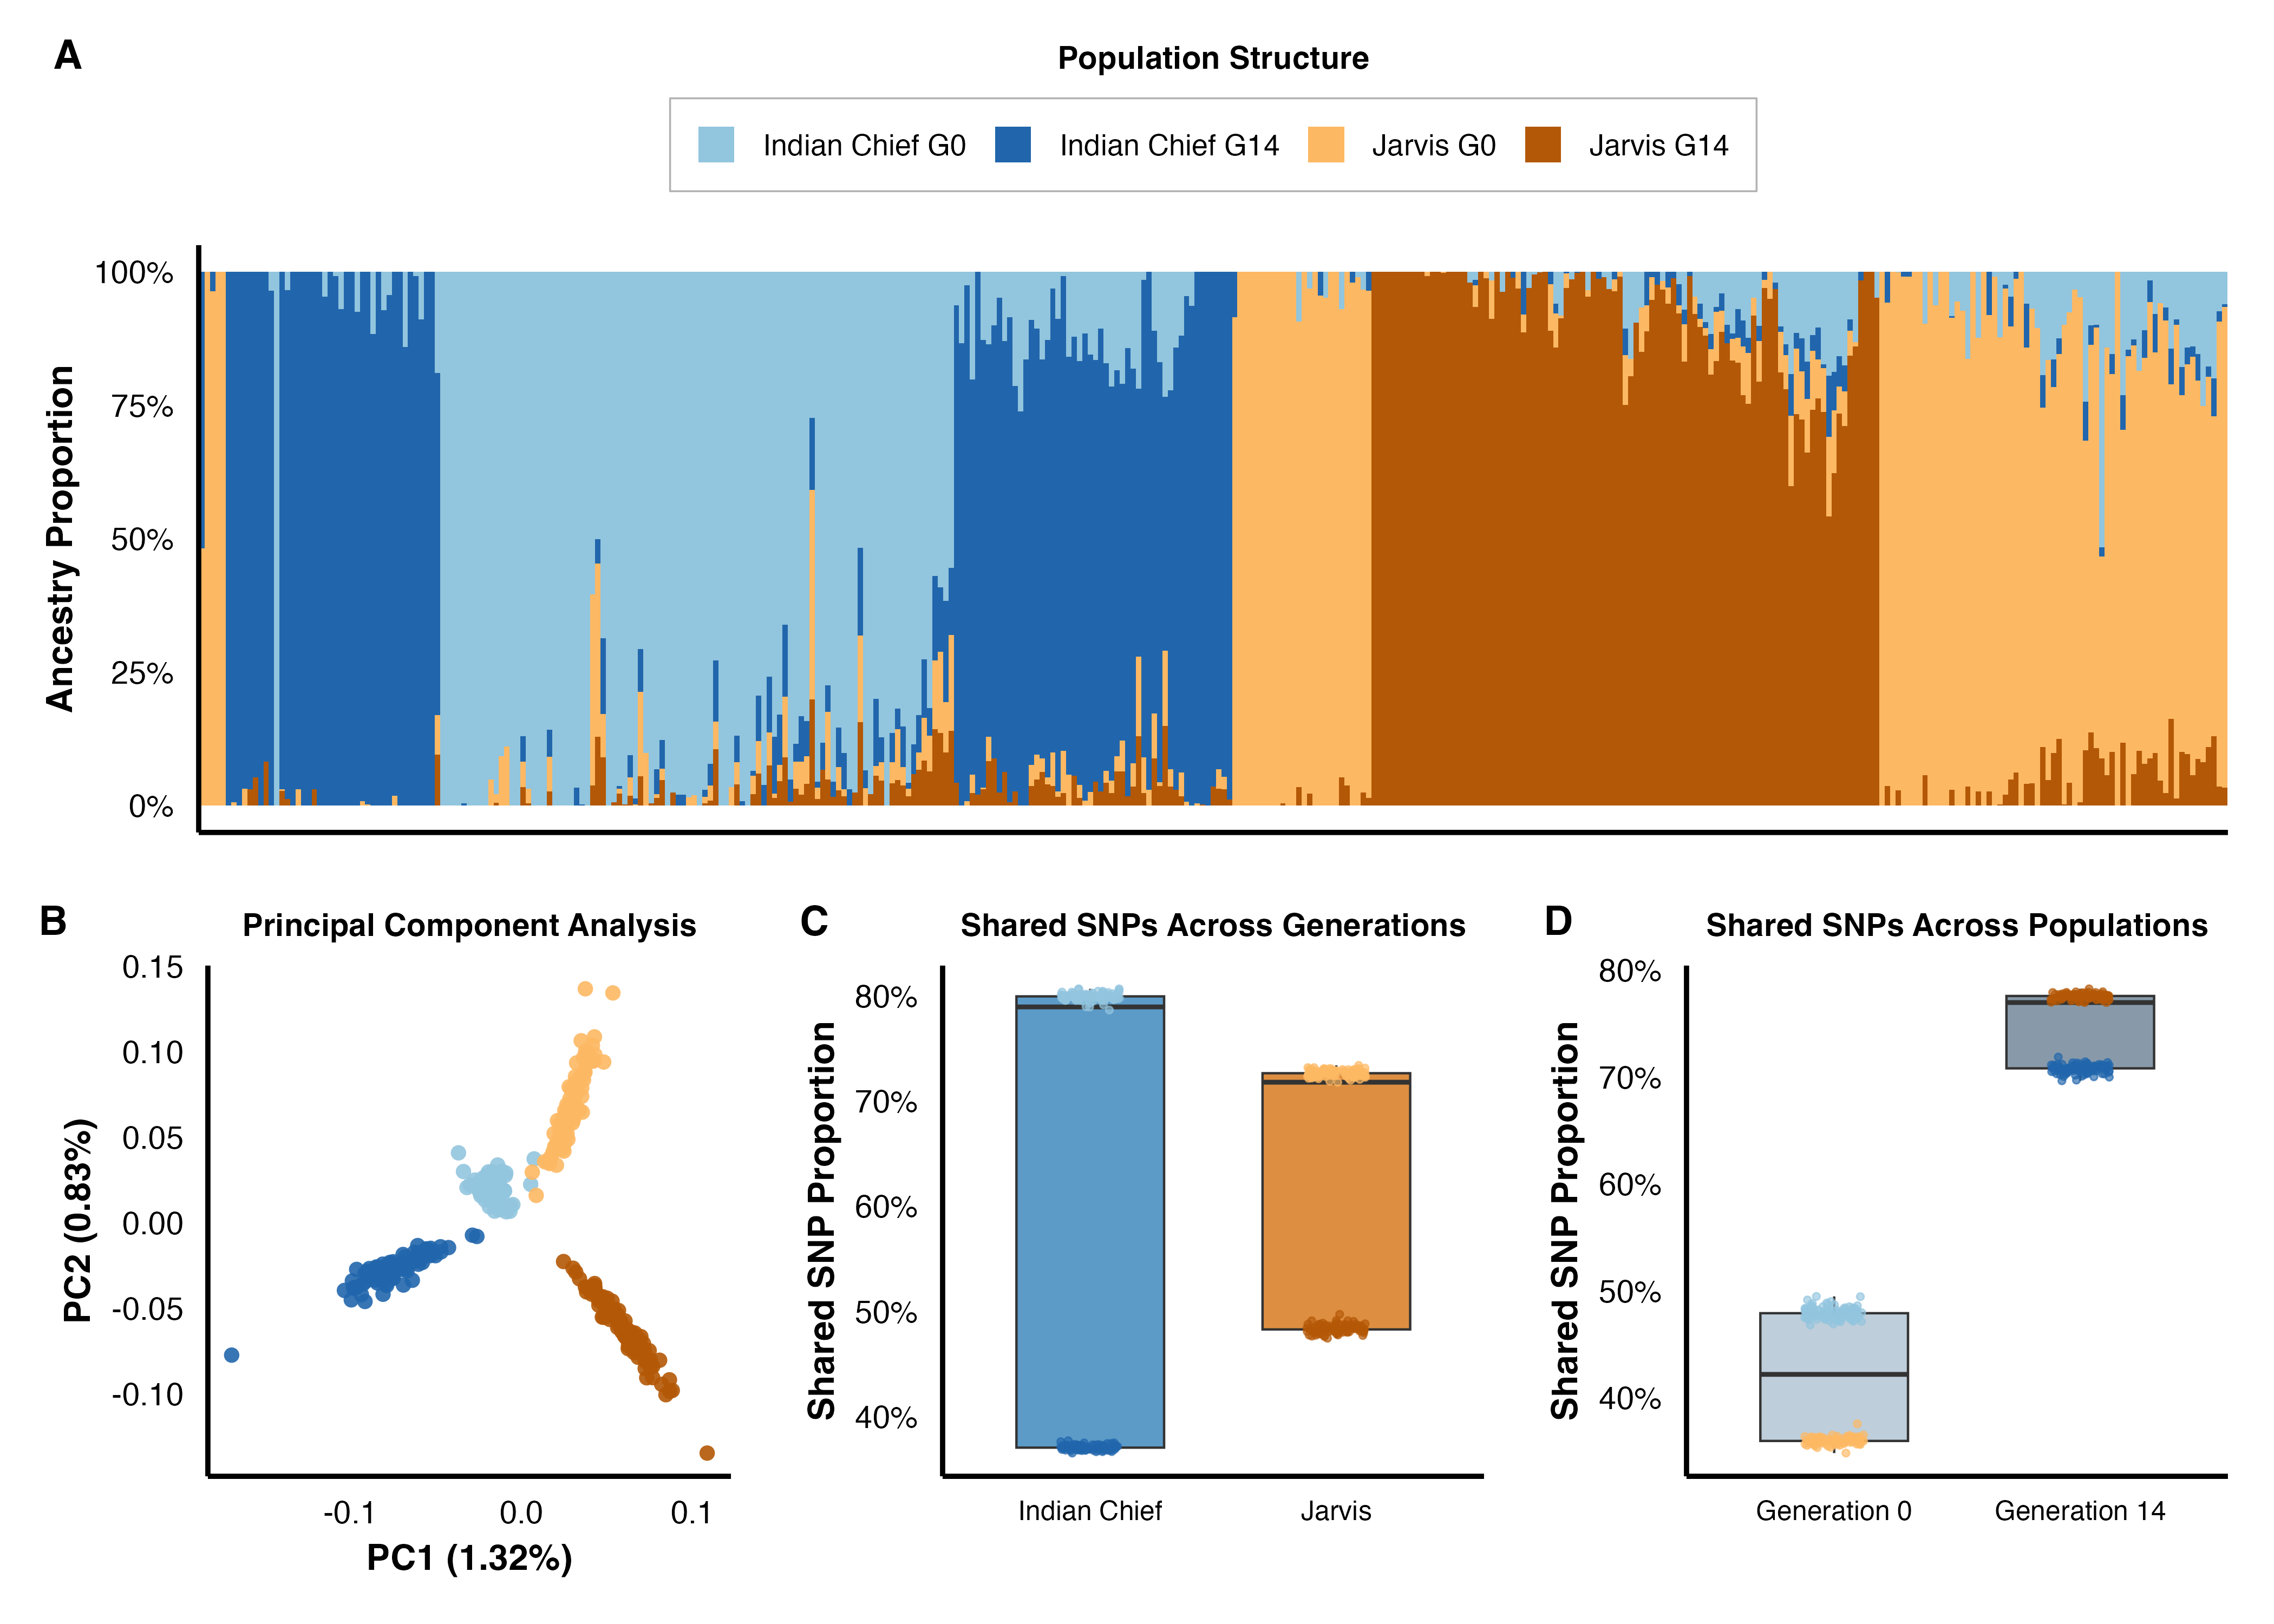
\includegraphics[width=0.9\linewidth]{Figs/main/Fig3.png}
    \caption{Skim sequencing reveals generation-specific genetic differentiation in Indian Chief and Jarvis. \textbf{A}, Population structure inferred from the LD-pruned SNP set, with ancestry proportions shown for Indian Chief Generation~0, Indian Chief Generation~14, Jarvis Generation~0, and Jarvis Generation~14. \textbf{B}, Principal component analysis of the same individuals and marker set. \textbf{C}, Proportion of SNPs shared across generations within each population. \textbf{D}, Proportion of SNPs shared across populations within each generation.}
    \label{fig:fig3}
\end{figure*}

Between populations, patterns differed from those within populations. Generation~14 individuals shared a higher proportion of SNPs between Indian Chief and Jarvis than did Generation~0 individuals, with mean proportions of ~0.742 and 0.420, respectively (Fig.~\ref{fig:fig3}D). Thus, long-term selection increased the fraction of alleles shared between the two selected populations, even though Indian Chief and Jarvis remained clearly differentiated in structure and PCA. Overall, 14 selection cycles markedly reshaped allele frequencies within each population, increased allelic overlap between generations, yet preserved broad genomic differentiation between Indian Chief and Jarvis.


\subsection{Selection scans in Indian chief and Jarvis reveal population-specific protein-turnover and amino acid metabolism candidates}

To identify genomic regions that differentiated across 14 cycles of reciprocal recurrent selection, we compared Cycle~0 and Cycle~14 within Indian Chief and Jarvis using three complementary population-genetic statistics: $F_{ST}$, $\Delta$ Tajima's~$D$, and $\log_2(\pi_{C14}/\pi_{C0})$. Because this breeding history spans only 14 selection cycles, we used an exploratory empirical threshold rather than a strict significance framework, reasoning that recent selection may produce moderate but coordinated shifts rather than extreme sweep signals. Candidate windows were therefore defined using the top 5\% of $F_{ST}$ values together with the bottom 5\% of $\Delta$ Tajima's~$D$ and $\log_2(\pi_{C14}/\pi_{C0})$ values, and were retained only when all three statistics supported the same window. This concordance criterion was used to prioritize regions showing consistent evidence of differentiation, allele-frequency change, and reduced diversity across selection cycles.

In parallel, GWAS in the NAM panel identified proline as a major axis of amino acid variation. We therefore tested whether genes from the concordant $F_{ST}$, nucleotide-diversity, and Tajima's $D$ scans overlapped genes associated with proline concentration in NAM.Using an exploratory empirical 5\% threshold for each statistic, we retained only windows supported jointly by $F_{ST}$, nucleotide diversity, and Tajima's $D$. This concordance filter yielded 97 candidate windows in Indian Chief (312 genes) and 126 candidate windows in Jarvis (357 genes). Of 41 proline-associated GWAS genes detected at $-\log_{10}(p) \ge 7$, only one overlapped the Indian Chief all-three candidate set and none overlapped the Jarvis set. The overlapping Indian Chief gene, \textit{Zm00001eb372060}, encodes an autophagy-related protein (Supplementary Table~\ref{tab:selection_candidate_go}), providing a mechanistically plausible link between population differentiation and altered nitrogen recycling, given autophagy’s role in degrading and recycling cellular proteins and organelles during senescence and nutrient remobilization.


The Indian Chief concordant candidate set showed several functional themes consistent with the observed FAA remodeling. Regions supported jointly by $F_{ST}$, nucleotide diversity, and Tajima's $D$ contained multiple genes associated with protein turnover and cellular recycling, including E3 ubiquitin ligases, ubiquitin-like proteases, ubiquitin-conjugating enzymes, cysteine and aspartyl proteases, and autophagy-related proteins. Notable examples included \textit{Zm00001eb372060}, \textit{Zm00001eb287690}, and \textit{Zm00001eb352300}, annotated as autophagy-related proteins; \textit{Zm00001eb372010}, annotated as a ubiquitin-like protease; \textit{Zm00001eb214780}, annotated as a senescence-specific cysteine protease; and \textit{Zm00001eb287650}, annotated as an aspartyl protease. These functions are relevant because protein degradation and autophagy can recycle cellular proteins and organelles into amino acid pools during senescence and nutrient redistribution.

The same Indian Chief candidate set also contained genes linked to nitrogen transport and amino acid metabolism, including \textit{Zm00001eb214890}, annotated as an ammonium transporter; \textit{Zm00001eb287950}, annotated as an NRT1/PTR-family transporter; \textit{Zm00001eb214770}, annotated as an NADP-specific glutamate dehydrogenase; and \textit{Zm00001eb287580}, associated with histidine biosynthesis. Together with the FAA data, these candidates suggest that Indian Chief Cycle~14 underwent broader remodeling of nitrogen recycling, amino acid interconversion, and protein turnover pathways rather than selection on a single canonical proline pathway.

The broader Indian Chief $F_{ST}$ outlier set reinforced the amino acid and N-remobilization themes suggested by the concordant scan. Several candidates were directly connected to amino acid metabolism or transport, including \textit{Zm00001eb214360}, annotated as aspartate-semialdehyde dehydrogenase with roles in amino acid, lysine, methionine, threonine, and isoleucine biosynthesis; \textit{Zm00001eb294790}, annotated as threonine synthase; \textit{Zm00001eb060520}, annotated as glutamate dehydrogenase with amino acid metabolism, glutamate catabolism, and cellular response to nitrogen starvation annotations; and amino acid transporters such as \textit{Zm00001eb052860}, \textit{Zm00001eb357860}, \textit{Zm00001eb380520}, and \textit{Zm00001eb427800}. The presence of aspartate-family and glutamate-related candidates is notable given the significant reduction in Asp and Glu fractions in Indian Chief Cycle~14, suggesting that selection-associated differentiation may involve remodeling of central amino acid interconversion and transport pathways rather than only proline accumulation.

The Indian Chief $F_{ST}$ candidates also included multiple genes associated with protein turnover, senescence, autophagy, and cellular recycling. These included ubiquitin and proteasome-related genes such as \textit{Zm00001eb397770}, \textit{Zm00001eb432790}, \textit{Zm00001eb397480}, \textit{Zm00001eb414990}, \textit{Zm00001eb415500}, \textit{Zm00001eb225210}, \textit{Zm00001eb204890}, and \textit{Zm00001eb380500}, as well as proteases including \textit{Zm00001eb066830}, \textit{Zm00001eb151510}, \textit{Zm00001eb317260}, \textit{Zm00001eb317270}, and \textit{Zm00001eb023280}. Autophagy- and vesicle-mediated recycling candidates were also present, including \textit{Zm00001eb151200}, annotated as autophagy-related protein 18f, and \textit{Zm00001eb420250}, annotated with autophagosome assembly and mitophagy. Together, these candidates suggest that Indian Chief selection-associated regions are enriched for pathways involved in protein degradation, amino acid release, and intracellular recycling, consistent with a model in which Cycle~14 FAA remodeling reflects broader changes in N recycling and amino acid allocation. 



\begin{table*}[ht]
\centering
\scriptsize
\caption{Overlap between SoilN or amino-acid GWAS genes and spline-based $F_{ST}$ outlier genes in Indian Chief (IC) and Jarvis (J). Traits shown are SoilN, Asp, Asn, Glu, Gln, and Proline. $F_{ST}$ genes were defined from spline windows with \texttt{fst\_outlier = Yes}. No overlapping genes were shared between IC and J for these traits.}
\label{tab:fst_gwas_overlap_ic_j}
\begin{tabular}{p{1.6cm}p{5.9cm}p{5.9cm}p{1.7cm}}
\hline
Trait & IC overlap genes & J overlap genes  \\
\hline
SoilN & Zm00001eb411350 & Zm00001eb276840; Zm00001eb276850; Zm00001eb276860 \\
Asp & None & Zm00001eb242960; Zm00001eb242970; Zm00001eb242980; Zm00001eb242990; Zm00001eb243000; Zm00001eb243010; Zm00001eb243020 \\
Asn & Zm00001eb060180; Zm00001eb060190; Zm00001eb101960; Zm00001eb101970; Zm00001eb101980; Zm00001eb162480; Zm00001eb287870 & Zm00001eb132940; Zm00001eb277110; Zm00001eb277130; Zm00001eb277140 \\
Glu & None & Zm00001eb131670; Zm00001eb131680; Zm00001eb237480; Zm00001eb237490 \\
Gln & Zm00001eb201180; Zm00001eb413150 & Zm00001eb012640; Zm00001eb012650; Zm00001eb012660 \\
Proline & Zm00001eb068910; Zm00001eb068930; Zm00001eb068940; Zm00001eb217140; Zm00001eb217150; Zm00001eb217160; Zm00001eb372060 & Zm00001eb131420 \\
\hline
\end{tabular}
\end{table*}


For Jarvis, the FAA phenotype was weaker and statistically underpowered because the Cycle~0 group contained only three biological samples. Total FAA abundance was numerically lower in Cycle~14 than in Cycle~0 (9.89 vs.\ 13.41; Wilcoxon rank-sum $p = 0.3583$; BH-adjusted $p = 0.6271$), and proline fraction also decreased numerically from 0.455 to 0.322 ($p = 0.1846$; BH-adjusted $p = 0.4307$). The N-rich FAA pool showed a similar numerical decrease from 2.35 to 1.80 ($p = 0.1846$; BH-adjusted $p = 0.4307$). By contrast, Asp fraction increased from 0.075 to 0.137 in Cycle~14. This increase was nominally significant before multiple-testing correction ($p = 0.0189$), but did not remain significant after BH correction ($p = 0.1323$). Thus, Jarvis showed a directional pattern toward reduced total FAA and proline representation, with a possible increase in Asp representation in the Cycle~14 FAA pool.

The Jarvis concordant selection-scan candidates provided a broader genomic context for this FAA pattern. Regions supported jointly by $F_{ST}$, nucleotide diversity, and Tajima's $D$ contained several genes related to protein turnover, protein stability, translation, and stress-associated metabolism. These included \textit{Zm00001eb210360}, annotated as an OTU-domain deubiquitinating enzyme; \textit{Zm00001eb146560}, an NPL4-like protein associated with ubiquitin-dependent protein catabolism; \textit{Zm00001eb175050}, a ubiquitin carboxyl-terminal hydrolase; \textit{Zm00001eb210720}, a 26S proteasome non-ATPase regulatory subunit; and \textit{Zm00001eb211020}, a BTB/POZ-domain protein annotated with protein ubiquitination. Jarvis also contained multiple ribosomal and translation-related candidates, including \textit{Zm00001eb210740}, \textit{Zm00001eb175100}, \textit{Zm00001eb211130}, \textit{Zm00001eb211010}, and \textit{Zm00001eb211090}, suggesting that selection-associated regions may involve protein synthesis and turnover balance rather than a single proline-specific pathway.

Additional Jarvis candidates were associated with stress responses, chloroplast or mitochondrial function, and transport processes. These included \textit{Zm00001eb210630}, annotated with endoplasmic-reticulum-associated degradation and unfolded-protein response; \textit{Zm00001eb210680}, annotated with response to endoplasmic reticulum stress; \textit{Zm00001eb211170}, associated with protein import into chloroplast stroma; \textit{Zm00001eb210890}, associated with thylakoid membrane organization and chloroplast protein insertion; and mitochondrial electron-transport candidates such as \textit{Zm00001eb384540}, \textit{Zm00001eb384490}, and \textit{Zm00001eb384430}. Together, these annotations suggest that Jarvis Cycle~14 differentiation may involve stress-associated protein quality control, organellar protein turnover, and energy metabolism. In contrast to Indian Chief, however, the Jarvis all-three candidate set did not point strongly to canonical proline biosynthesis or catabolism. The FAA and genomic data therefore support a more cautious model in which Jarvis may have shifted away from proline-dominated FAA composition, with possible Asp enrichment, through broader changes in protein turnover and organellar stress-response pathways.


The broader Jarvis $F_{ST}$ outlier set strengthened the view that selection-associated differentiation involved amino acid transport, protein turnover, and organellar stress pathways. Several candidates were directly related to amino acid metabolism or transport, including \textit{Zm00001eb231430}, annotated as aspartate--tRNA ligase; \textit{Zm00001eb237500}, annotated as D-amino-acid transaminase; \textit{Zm00001eb132750}, annotated as a lysine/histidine transporter-like protein; \textit{Zm00001eb159580}, annotated as a putative GABA transporter; and \textit{Zm00001eb389560}, annotated as GLUTAMINE DUMPER 5 with amino acid transport and regulation of amino acid export. These candidates are notable given the Jarvis FAA pattern, where Asp fraction was numerically higher in Cycle~14, while proline fraction was numerically lower. Although the FAA comparison was underpowered, the $F_{ST}$ candidates suggest that amino acid transport, aminoacylation, and amino acid interconversion may contribute to the altered FAA composition in Jarvis.

Jarvis $F_{ST}$ outliers also included several genes associated with protein turnover, autophagy, and protein quality control. These included \textit{Zm00001eb142210}, annotated as autophagy-related protein 18a; \textit{Zm00001eb210360} and \textit{Zm00001eb242070}, annotated as OTU-domain deubiquitinating enzymes; \textit{Zm00001eb130370}, annotated as a ubiquitin-conjugating enzyme; \textit{Zm00001eb072830}, \textit{Zm00001eb073090}, and \textit{Zm00001eb242020}, annotated as RING/U-box E3 ubiquitin-related proteins; \textit{Zm00001eb231490}, annotated as a proteasome alpha subunit; and \textit{Zm00001eb128130}, annotated as a 26S proteasome regulatory subunit. Additional candidates such as \textit{Zm00001eb424420}, a UBX-domain protein associated with autophagosome assembly and proteasome-mediated ubiquitin-dependent protein catabolism, further support a role for protein recycling. Together, these genes suggest that Jarvis differentiation may involve protein degradation and recycling pathways that could influence FAA availability and N redistribution.

The Jarvis $F_{ST}$ candidate set also contained genes related to chloroplast, mitochondrial, and stress-response functions. These included \textit{Zm00001eb150810}, annotated with response to water deprivation, heat acclimation, hyperosmotic salinity response, photooxidative stress, and photosystem I assembly; \textit{Zm00001eb237270}, annotated as tocopherol cyclase with oxidative-stress and phloem sucrose-loading annotations; \textit{Zm00001eb073200}, a mitochondrial mechanosensitive ion channel associated with oxidative-stress response; and mitochondrial or chloroplast translation and electron-transport genes such as \textit{Zm00001eb210740}, \textit{Zm00001eb160260}, \textit{Zm00001eb384540}, and \textit{Zm00001eb237310}. Overall, the Jarvis $F_{ST}$ scan did not point to a single canonical proline biosynthesis or catabolism locus. Instead, it highlighted amino acid transport, Asp-related translation machinery, protein turnover, and organellar stress-response pathways, consistent with a cautious model in which Jarvis Cycle~14 may show reduced proline representation and increased Asp representation through broader remodeling of amino acid and N-recycling systems.




\begin{figure*}[ht!]
    \centering
    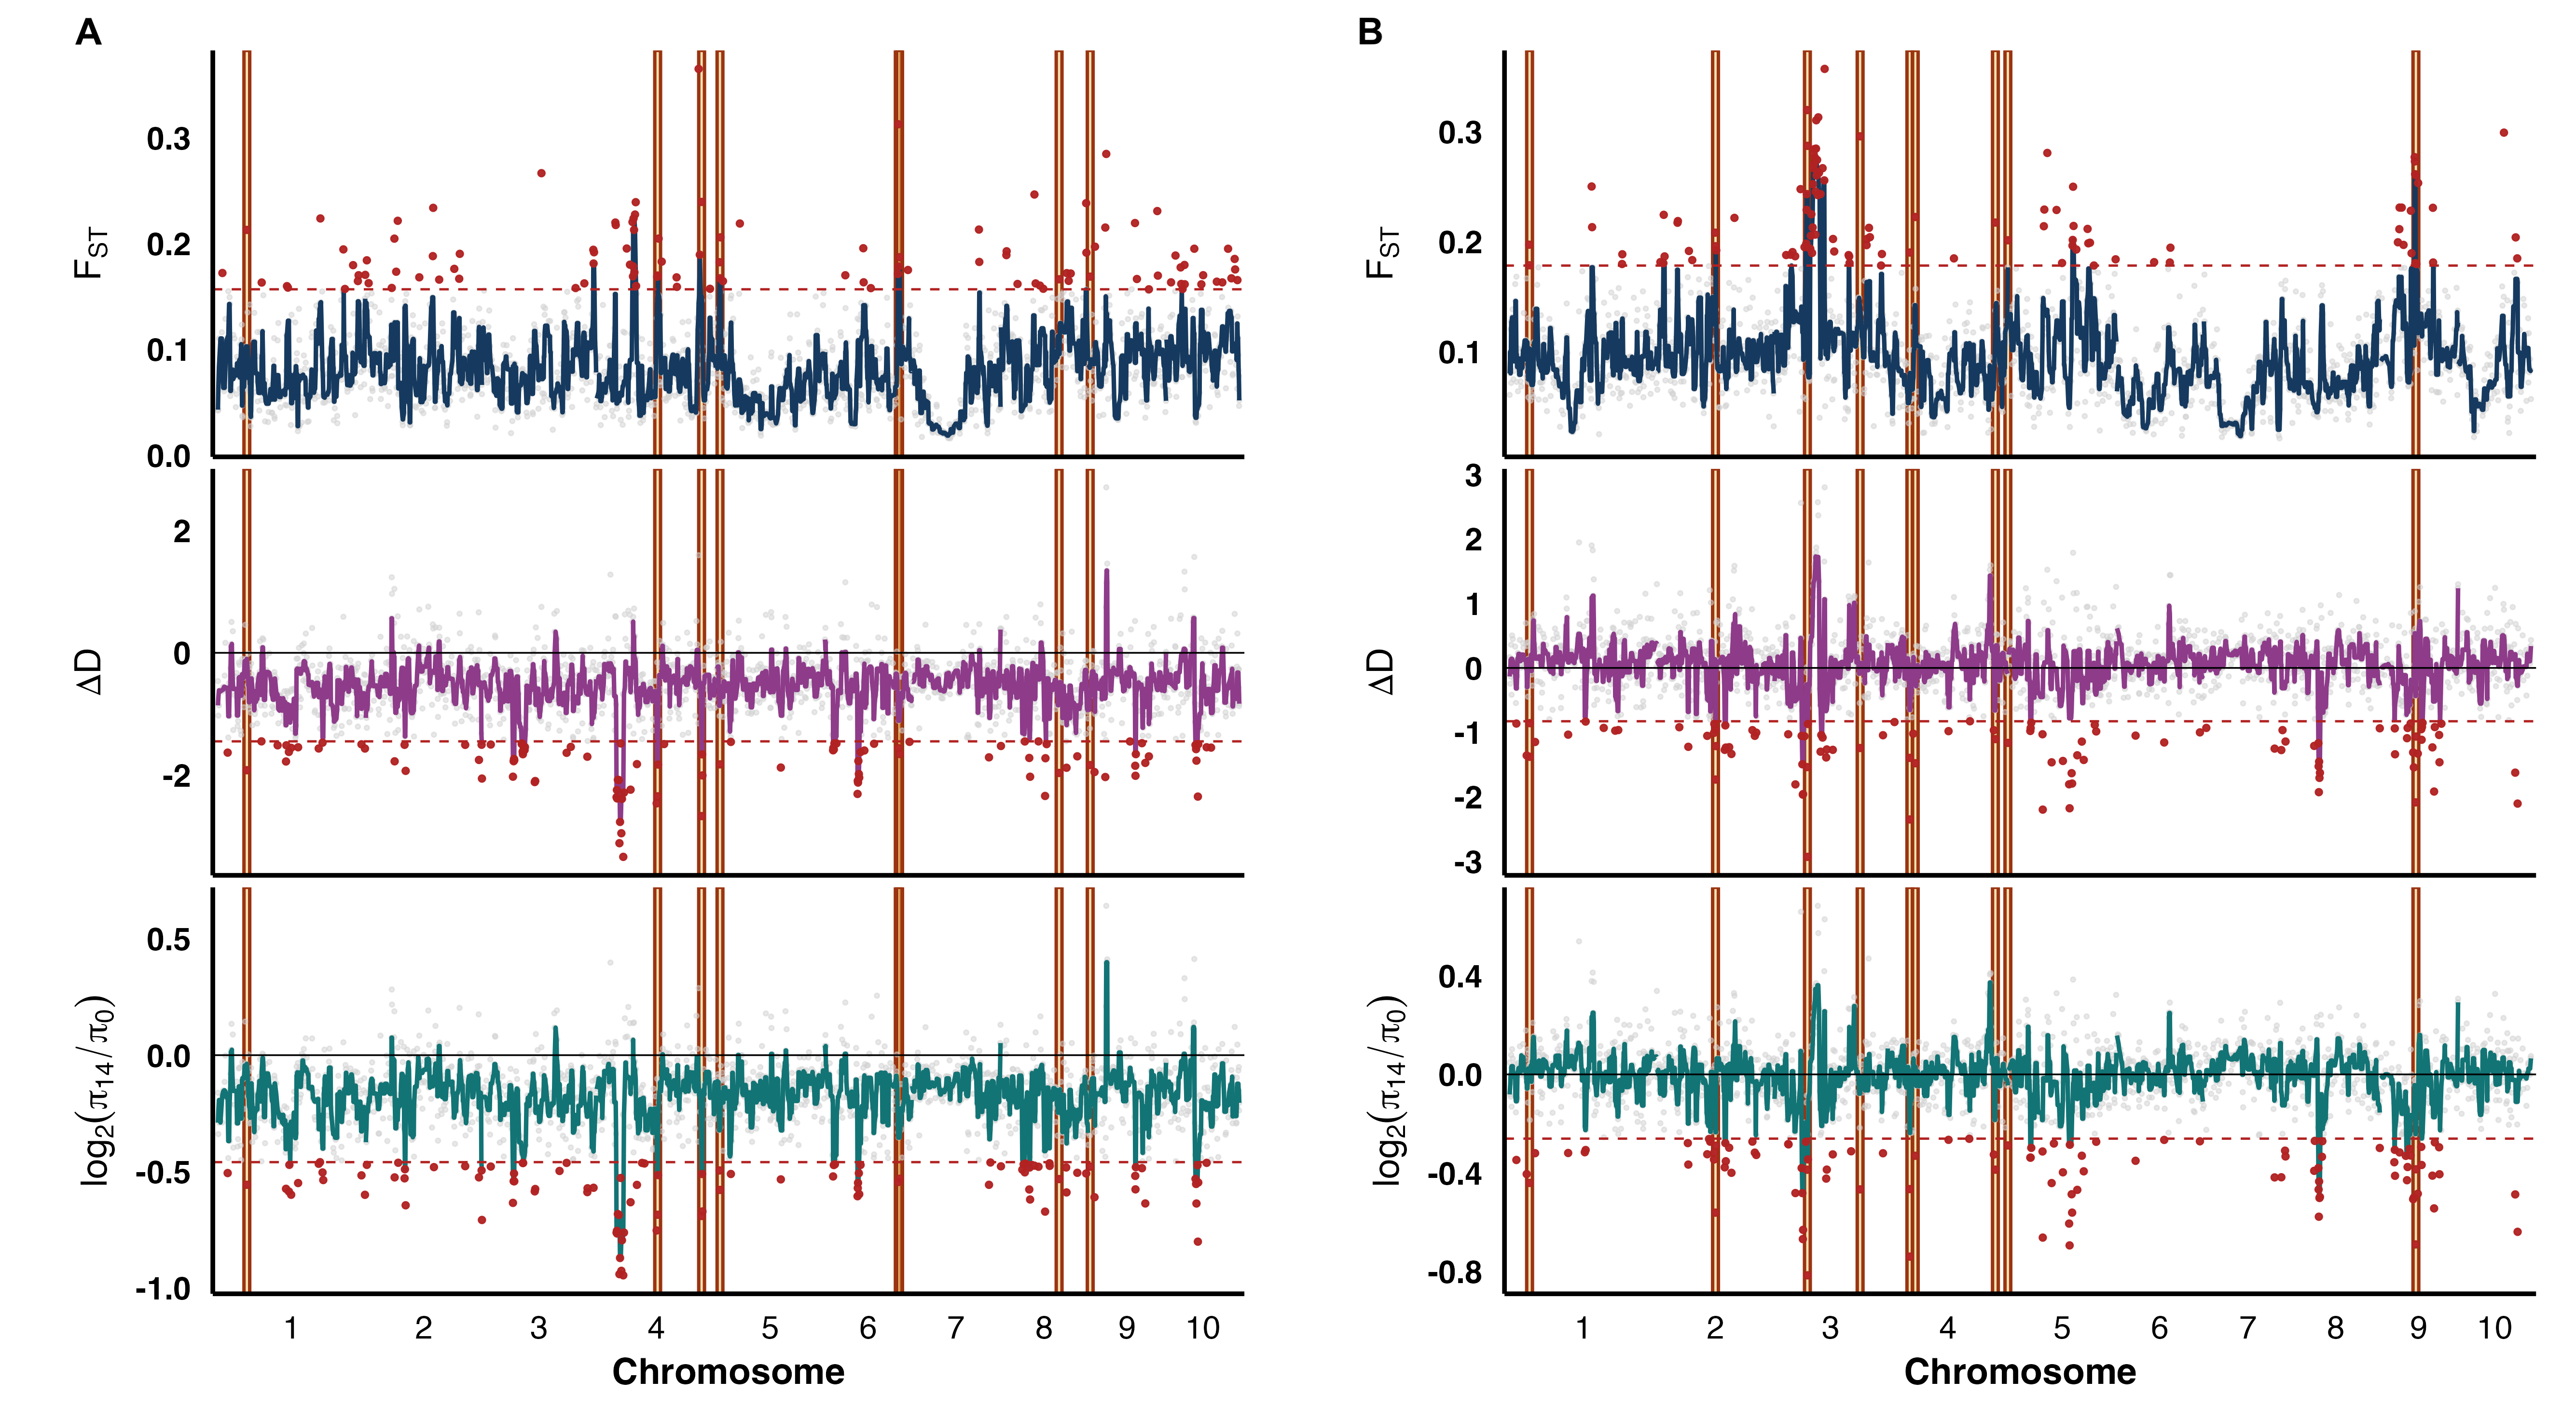
\includegraphics[width=0.8\textwidth]{Figs/main/Fig5.png}
    \caption{Genome-wide scans of population differentiation and diversity changes between Generation~0 and Generation~14 in Indian Chief and Jarvis. \textbf{A}, Indian Chief. \textbf{B}, Jarvis. Tracks show $F_{ST}$, $\Delta$ Tajima's $D$, and $\log_2(\pi_{G14}/\pi_{G0})$ across the genome. Shaded vertical bands indicate candidate regions supported by all three summary statistics under the empirical 5\% threshold scheme, defined as the top 5\% of $F_{ST}$ values together with the bottom 5\% of $\Delta$ Tajima's $D$ and $\log_2(\pi_{G14}/\pi_{G0})$ values.}
    \label{fig:fig5}
\end{figure*}


\section{Methods}\label{methods}

\subsection{Germplasm used}
\subsubsection{Maize Landraces}
The maize landraces discussed by Romero Navarro et al. (2017, ref) come from the CIMMYT International Germplasm Bank collection, which contains over 24,000 accessions of traditional maize varieties primarily from North, Central, and South America. They characterized a core collection of 3,511 genotypes based on availability of accurate geographic coordinates and complete environmental data for their collection locations. These landraces are genotyped using genotyping-by-sequencing (GBS) at about 2X coverage, with SNP calling and imputation for analysis. The population represents a geographically and genetically diverse panel that serves as an important resource for studying environmental adaptation like soil nitrogen (N) availability.
How were they grown when they were phenotyped?

\subsubsection{Indian Chief and Jarvis (IC and J)  }
We worked with two open-pollinated maize populations Indian Chief (IC) and Jarvis (J) from Moll et al. (1994, ref) that underwent reciprocal recurrent selection for 14 generations for grain yield. Beginning from base populations (G₀), each cycle involved intercrossing the best families selected on hybrid (ICxJ) performance and advancing through a selfed recombination nursery. 
How were they grown in 2025? This is relevant for the AA profiling I am doing 

\subsubsection{Indian Chief and Jarvis recurrent-selection populations}

We used two open-pollinated maize populations, Indian Chief (IC) and Jarvis Golden Prolific (J), from the recurrent-selection experiment described by \citet{Moll1994}. These populations underwent 14 cycles of reciprocal recurrent selection for grain yield. In this scheme, parents within each population were selected based on the performance of their hybrid progeny in the IC~$\times$~J population, and selfed progeny from the selected parents were intermated to generate the next selection cycle. For the present study, individuals from the base populations, Cycle~0 (C0), and the selected populations, Cycle~14 (C14), were analyzed for both Indian Chief and Jarvis.

For amino acid profiling, IC\_C0, IC\_C14, J\_C0, and J\_C14 plants were grown in 2025 at \textit{[insert location/field site]}. Plants were grown using a \textit{[insert experimental design; e.g., randomized complete block design]} with \textit{[insert number]} biological replicates per population--cycle group. Standard agronomic management was applied throughout the season, including \textit{[insert planting date, spacing, fertilizer regime, irrigation/rainfed condition, and pest/weed management if relevant]}. Tissue for free amino acid profiling was collected from \textit{[insert tissue; e.g., grain, leaf, seedling tissue]} at \textit{[insert developmental stage or harvest time]}, immediately frozen or dried according to the extraction protocol, and stored at \textit{[insert storage condition]} until metabolite analysis.


\subsubsection{The Goodman-Buckler Maize Association Panel}
The Goodman-Buckler maize association panel (Flint-Garcia et al., 2005)  was grown at Genetics Farm near Columbia Missouri in 2017 and 2018 in two replicates each, in a randomized complete block design. Of the 282 lines in this panel, only 279 were grown successfully. 13 kernels of each line were planted in a 10 foot row and self-pollinated. At full physiological maturity, the pollinated ears were harvested, husk leaves were removed, and were subsequently dried at 105 degrees fahrenheit and <20 relative humidity for 5 days to remove moisture from the grain. Ears from each line in each rep and year were shelled and bulked to form four representative composite grain samples for each of the 279 lines. For phenotypic evaluation, 25 random seeds were selected from each bulked sample to be ground and prepared for amino acid extraction and quantification

\subsubsection{Bi-parental Mapping Population}
The bi-parental QTL mapping population was developed by crossing the two inbred lines of the Goodman-Buckler Association Panel with the lowest and highest free Asn accumulation in the grain, B64 and CML14, respectively. F2:3 families were grown in two complete randomized blocks in 2024 at Genetics Farm near Columbia Missouri. For each plot, 13 kernels were planted in a 10-foot row and sib-pollinated to produce three ears. At full physiological maturity, the pollinated ears were harvested, husk leaves were removed, and ears were subsequently dried at 41 degrees Celsius and 20\% relative humidity for 5 days to remove moisture from the grain. From each ear, 10 representative kernels were sampled then bulked, ground, and prepared for amino acid extraction and quantification.


\subsection{Phenotypic Evaluation}
\subsubsection{Grain/Stover Nitrogen}
Grain and stover N concentration for all IC and J lines was determined for the base generation (G₀) and the 14ᵗʰ cycle of selection (G₁₄) by Moll et al, (1994, ref). At a high fertilizer rate of 224 kgNha⁻¹, the J14 produced heavier kernels and a higher grain N concentration than the original J0 line. Post anthesis uptake from the soil supplied almost all of that extra N while the amount of nitrogen remobilised from stover to grain remained unchanged. The I14 behaved differently though. Vegetative biomass increased, but grain weight and grain N concentration stayed at the G₀ level. Loss of nitrogen from stover after flowering fell below that of the baseline, so more N was retained in stems and leaves and less reached the grain. Fourteen cycles of selection therefore raised grain N in J by drawing in more N after flowering, whereas the IC diverted N toward vegetative tissue and left grain N unchanged (ref).

\subsubsection{Soil Nitrogen}
The analyzed phenotypes include total N in the soil (TN) and nitrate deposition (NHx, which includes NH3 and NH4+). N data were derived from the top 0-5 cm of the soil, representing the active root zone for nutrient uptake, using ISRIC data sets (International Soil Reference and Information Center). Historical nitrate deposition data (NHx) from 1983 was also sourced from ISRIC to understand its relationship with nutrient uptake. 

\subsubsection{Amino Acid Profiling}
PBAAs were extracted and quantified as described in Yobi and Angelovici (2018). This protocol utilizes microscale protein hydrolysis and absolute quantification using multiple reaction monitoring-based liquid chromatography–tandem mass spectrometry detection. During acid hydrolysis, Gln and Asn are converted into Glu and Asp, respectively. Therefore, we denote both Gln and Glu as Glx and Asn and Asp as Asx. During the extraction, Trp and Cys were fully destroyed and Gly was poorly detected, therefore these three amino acids were excluded from the dataset. In total, 15 PBAAs were analyzed to represent 17 PBAAs. FAAs were extracted and quantified as described in (Gu et al., 2007). Unlike the protocol above, all 20 proteinogenic amino acids were independently and successfully detected using UPLC-MS/MS.


\subsection{Sequencing and genotyping}

\subsubsection{Indian Chief and Jarvis}

Genomic DNA was isolated from young leaf tissue of individuals from four reciprocal recurrent-selection population--cycle groups: Indian Chief base generation (I01), Indian Chief Cycle~14 (I14), Jarvis base generation (J01), and Jarvis Cycle~14 (J14). Each group initially included 96 individuals, for a total of 384 samples. These populations were generated after 14 cycles of reciprocal recurrent selection for increased grain yield \citep{Moll1994}. Paired-end Illumina libraries were constructed and sequenced as 2~$\times$~150~bp reads on a NovaSeq~6000 platform. Raw base-call files were demultiplexed with \texttt{fqtk} v0.3.1, yielding one 96-sample plate for each population--cycle group (Supplementary Table~S1).

Adapter trimming and quality filtering used \texttt{fastp} v0.23.4, and read quality was assessed with \texttt{FastQC} v0.12.1. Trimmed reads were aligned to the B73 NAM reference genome RefGen\_v5 (GCF\_902167145.1) with \texttt{BWA-MEM} v0.7.18. Alignments were coordinate-sorted, duplicates were collapsed with \texttt{Picard MarkDuplicates} v3.1.1, and read groups were standardized with \texttt{Picard AddOrReplaceReadGroups}. Variant discovery followed the GATK Best Practices joint-genotyping workflow using \texttt{GATK} v4.5.0.0. Joint genotyping was performed per chromosome with \texttt{CombineGVCFs} and \texttt{GenotypeGVCFs}, generating 10 per-chromosome VCFs that were merged into a cohort VCF with 80,728,251 raw variant sites. Five low-quality samples (I14\_A07, I14\_B06, I14\_D05, I14\_F12, J14\_H11) were removed, leaving 379 genomes for population-genomic analysis (Supplementary Table~S1). Genome-wide coverage was estimated with \texttt{Picard CollectWgsMetrics}: mean coverage was 0.28$\times$ for I01, 0.38$\times$ for I14, 0.32$\times$ for J01, and 0.37$\times$ for J14, consistent with low-pass skim sequencing (Supplementary Fig.~S1). SNPs and indels were filtered with GATK hard-filtering criteria, yielding 59,199,563 high-confidence variants, including 52,543,238 SNPs and 6,656,325 indels across the 10 maize chromosomes and scaffolds (Supplementary Table~S2). The filtered SNP set was used for downstream population-genomic analyses.



\subsubsection{The Goodman-Buckler maize association panel}
The Goodman-Buckler maize association panel had been previously genotyped with both the Illumina MaizeSNP50 BeadChip (Cook et al., 2012) and with genotyping-by-sequencing (GBS) method (Elshire et al., 2011) as described in (Lipka et al., (2013). We filtered SNPs by minor allele frequency greater than 0.05 prior to analysis. HAPPI GWAS utilizes GAPIT MLMM, FarmCPU, and BLINK models to conduct univariate GWAS. Following the GWAS, we used false discovery rate (FDR) to correct the multiple hypothesis testing problem at 5\%. Using the Maize AGP\_V5, we identified candidate genes within 25kb on either side of SNPs with a p value of less than 0.001. 

\subsubsection{Bi-parental Mapping Population}
Leaf tissues were collected from F2 plants and lyophillized prior to DNA extraction and genotyping using the mid-density temperate corn panel by Agriplex Genomics (Cleveland, OH).

\subsection{Population-genomic analyses}

\subsubsection{Genotype-likelihood framework}

Population-genomic statistics were estimated using ANGSD v0.941 \citep{Korneliussen2014}, which is appropriate for low-coverage sequencing because it uses genotype likelihoods rather than hard genotype calls. Analyses were performed separately for Indian Chief Cycle~0 (IC\_C0), Indian Chief Cycle~14 (IC\_C14), Jarvis Cycle~0 (J\_C0), and Jarvis Cycle~14 (J\_C14). The same read- and base-level filtering parameters were applied across all population--cycle groups to ensure comparable estimates among contrasts.

For each population--cycle group, site allele-frequency likelihoods were estimated with ANGSD and stored as SAF files. Folded one-dimensional site-frequency spectra were inferred with \texttt{realSFS} for within-population analyses, because a reliable ancestral allele state was not assumed. For pairwise analyses, joint two-dimensional site-frequency spectra were estimated from the corresponding SAF files using \texttt{winsfs}, a window-EM SFS estimator, to improve computational efficiency. These joint spectra were then used as priors for downstream $F_{ST}$ estimation.

\subsubsection{Population differentiation using $F_{ST}$}

Genetic differentiation between ancestral and selected cycles was quantified using the ANGSD/\texttt{realSFS} $F_{ST}$ workflow. Pairwise $F_{ST}$ was estimated separately for the IC\_C0 versus IC\_C14 and J\_C0 versus J\_C14 contrasts. For each contrast, the joint two-dimensional site-frequency spectrum was first estimated using \texttt{winsfs} from the corresponding SAF files and then supplied as the prior to \texttt{realSFS fst index}. Windowed $F_{ST}$ values were summarized across the genome using 100~kb sliding windows with a 10~kb step size. The top 1\% of windows from each contrast were treated as high-differentiation outliers and retained for downstream candidate-region annotation.

\subsubsection{Nucleotide diversity}

Within-population nucleotide diversity was estimated separately for IC\_C0, IC\_C14, J\_C0, and J\_C14. Population-scaled theta estimates were computed from the folded one-dimensional site-frequency spectrum using \texttt{realSFS saf2theta}. Nucleotide diversity ($\pi$) was then summarized across the genome using \texttt{thetaStat do\_stat}. Windowed $\pi$ estimates were calculated in 100~kb sliding windows with a 10~kb step size, matching the windowing scheme used for the $F_{ST}$ scans. Windows showing strong reductions in nucleotide diversity in Cycle~14 relative to Cycle~0 were retained as candidate regions consistent with selection-associated loss of variation.

\subsubsection{Tajima's $D$}

Tajima's $D$ was estimated for each population--cycle group using the same theta-based ANGSD workflow. Folded one-dimensional site-frequency spectra were used to compute theta estimates with \texttt{realSFS saf2theta}, and Tajima's $D$ was summarized with \texttt{thetaStat do\_stat}. Values were calculated in 100~kb sliding windows with a 10~kb step size. Windows with extreme Tajima's $D$ values were retained as candidate regions reflecting departures from neutral allele-frequency expectations, including possible selection-associated shifts in the site-frequency spectrum.

\subsubsection{Candidate window annotation}

Candidate windows from the $F_{ST}$, nucleotide diversity, and Tajima's $D$ analyses were intersected with the maize reference gene annotation \textit{[insert annotation version]}. Genes overlapping or located near candidate windows were retained as candidate genes. Candidate lists from the three statistics were then compared within Indian Chief and Jarvis to identify genes supported by multiple population-genomic signals.





\subsubsection{Genome-wide association Studies}
\paragraph{Environment GWAS}
GWAS was performed on maize landraces (n = 3,511) using four GWAS models: MLM, MLMM, BLINK and FarmCPU. Approximately 495,755 SNPs for maize landraces. The maize genotype was based on the Zm-B73-REFERENCE-NAM-5.0 genome assembly. Candidate genes located within 25 kb maize landraces were identified using the MaizeGDB, Phytozome, and Arabidopsis databases. 

\paragraph{Metabolite GWAS}
Using the same pipeline described above for the envGWAS, we performed metabolite GWAS using the Goodman-Buckler Association Panel (n-278). In total, XXX SNPs were used to evaluate 110 traits for FAAs and 77 traits for PBAAs including absolute composition, total composition, relative composition, and various biochemical ratios. Prior to analysis, best linear unbiased predictions or BLUPs were calculated for each trait. For the metabolite GWAS, we used a GAPIT pipeline based on Holistic Analysis with Pre- and Post-Integration, or HAPPI GWAS. This pipeline, as described in (Slaten et al., 2020), removes outliers, optimizes transformation, and calculates BLUPs prior to the association study. 

To estimate the nitrogen content of the Goodman-Buckler maize association panel, we calculated the respective percentage of mass occupied by nitrogen in the 20 proteinogenic amino acids. Across the 4 composite samples, we multiplied the quantity of each amino acid in μg/mg by the calculated \% nitrogen mass for that amino acid to solve for the  quantity of nitrogen in μg/mg. We added the totals for each of the 20 proteinogenic amino acids together for the free amino acids as well as the quantified protein bound amino acids to find total approximated nitrogen content in each composite sample. 

\[
\%N_X =
\left(
\frac{n_{N,X}\times M_N}{M_X}
\right)\times 100
\]

where,
\[
M_X = \text{molar mass of amino acid } X
\]

\[
M_N = \text{molar mass of nitrogen}
\]

\[
n_{N,X} = \text{number of nitrogen atoms in amino acid } X
\]

Finally,
\[
N_X\;(\mu g/mg) =
\left(
\frac{n_{N,X}\times M_N}{M_X}
\right)
\times AA_X\;(\mu g/mg)
\]



We used these total proxy nitrogen (TPN) amounts for each composite sample to calculate the Best Linear Unbiased prediction (BLUP) before performing the GWAS as described above. We used a false discovery rate (FDR) to correct the multiple hypothesis testing problem at 5\%. Using the MaizeMine tool on MaizeGDB, we identified candidate genes within 100kb on either side of SNPs with a p value of less than 0.001. 

\paragraph{Quantitative Trait Loci Mapping}
We began with 2490 markers in total and following filtering of failed, monomorphic, and heterozygous markers 611 were used for the analysis. Markers were re-coded to be compatible with the r/qtl package used for mapping. Each allele was re-coded to AA to correspond with the allele associated with B64, BB for CML14, and AB if heterozygous. Best Linear Unbiased Predictions of absolute free aspartate content were calculated and used to construct the genetic map. To ensure quality of the genetic map, markers with more than 10\% inconclusive genotyping results were excluded and segregation ratios were checked to identify and remedy potential switched alleles. Linkage groups were formed by calculating max recombination fraction at 0.35 and minimum LOD at 15. Ultimately, one linkage group required manual separation and subsequent re-calculation of recombination fraction and LOD to produce an accurate genetic map to reflect the 10 chromosomes of maize. QTL scans were performed and significance thresholds were established at a=0.05 using 1000 permutations and Haley-Knott regression.

\section{Data availability}
All scripts and parameter files used in the pipeline are available at the github repository: https://github.com/nirwan1265/Grain\_N\_remobilization.


\section{Discussion}\label{sec12}

Discussions should be brief and focused. In some disciplines use of Discussion or `Conclusion' is interchangeable. It is not mandatory to use both. Some journals prefer a section `Results and Discussion' followed by a section `Conclusion'. Please refer to Journal-level guidance for any specific requirements. 

\section{Conclusion}\label{sec13}

Conclusions may be used to restate your hypothesis or research question, restate your major findings, explain the relevance and the added value of your work, highlight any limitations of your study, describe future directions for research and recommendations. 

In some disciplines use of Discussion or 'Conclusion' is interchangeable. It is not mandatory to use both. Please refer to Journal-level guidance for any specific requirements. 

\backmatter

\bmhead{Supplementary information}

If your article has accompanying supplementary file/s please state so here. 

Authors reporting data from electrophoretic gels and blots should supply the full unprocessed scans for key as part of their Supplementary information. This may be requested by the editorial team/s if it is missing.

Please refer to Journal-level guidance for any specific requirements.

\bmhead{Acknowledgements}

Acknowledgements are not compulsory. Where included they should be brief. Grant or contribution numbers may be acknowledged.

Please refer to Journal-level guidance for any specific requirements.

\section*{Declarations}

Some journals require declarations to be submitted in a standardised format. Please check the Instructions for Authors of the journal to which you are submitting to see if you need to complete this section. If yes, your manuscript must contain the following sections under the heading `Declarations':

\begin{itemize}
\item Funding
\item Conflict of interest/Competing interests (check journal-specific guidelines for which heading to use)
\item Ethics approval and consent to participate
\item Consent for publication
\item Data availability 
\item Materials availability
\item Code availability 
\item Author contribution
\end{itemize}

\noindent
If any of the sections are not relevant to your manuscript, please include the heading and write `Not applicable' for that section. 

%%===================================================%%
%% For presentation purpose, we have included        %%
%% \bigskip command. Please ignore this.             %%
%%===================================================%%
\bigskip
\begin{flushleft}%
Editorial Policies for:

\bigskip\noindent
Springer journals and proceedings: \url{https://www.springer.com/gp/editorial-policies}

\bigskip\noindent
Nature Portfolio journals: \url{https://www.nature.com/nature-research/editorial-policies}

\bigskip\noindent
\textit{Scientific Reports}: \url{https://www.nature.com/srep/journal-policies/editorial-policies}

\bigskip\noindent
BMC journals: \url{https://www.biomedcentral.com/getpublished/editorial-policies}
\end{flushleft}

\begin{appendices}

\section{Section title of first appendix}\label{secA1}

An appendix contains supplementary information that is not an essential part of the text itself but which may be helpful in providing a more comprehensive understanding of the research problem or it is information that is too cumbersome to be included in the body of the paper.

\begin{figure*}[!htbp]
    \centering
    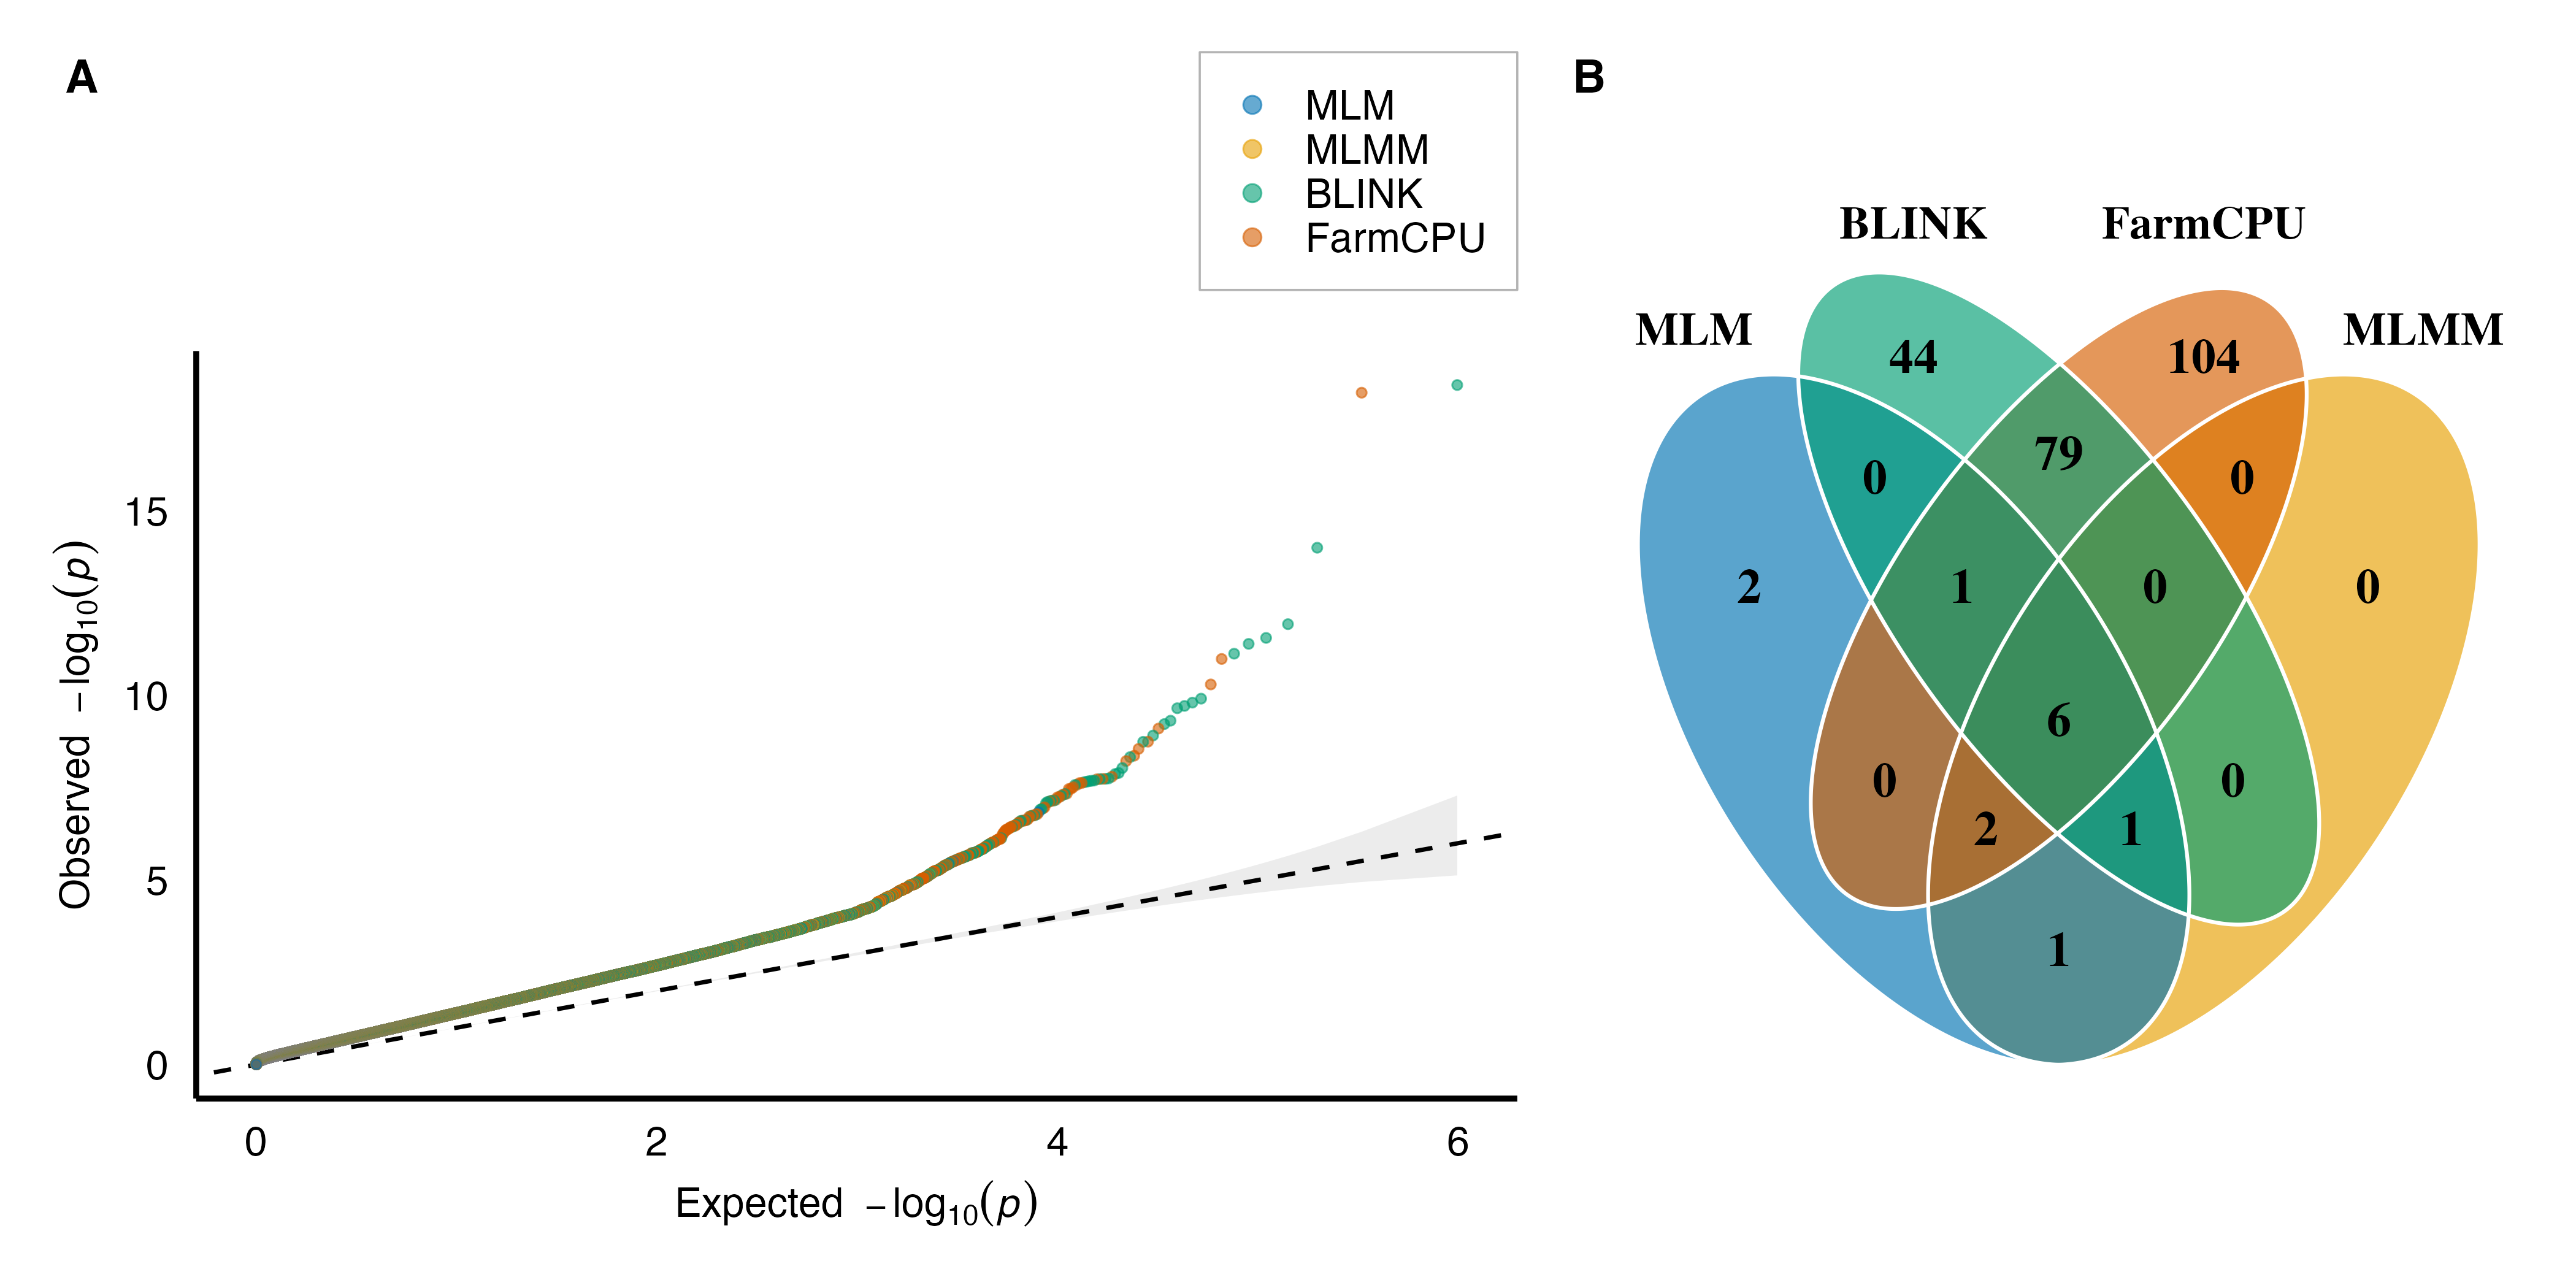
\includegraphics[width=\textwidth]{Figs/Supplementary/SuppFig_QQ_venn.png}
    \caption{Supplementary soil N GWAS diagnostics and model overlap. \textbf{A}, Quantile--quantile plot comparing expected and observed $-\log_{10}(p)$ values for the MLM, MLMM, BLINK, and FarmCPU models. \textbf{B}, Venn diagram showing overlap among models for loci exceeding the suggestive threshold used for comparison.}
    \label{fig:supp_soiln_qq_venn}
\end{figure*}

\begin{figure*}[!htbp]
    \centering
    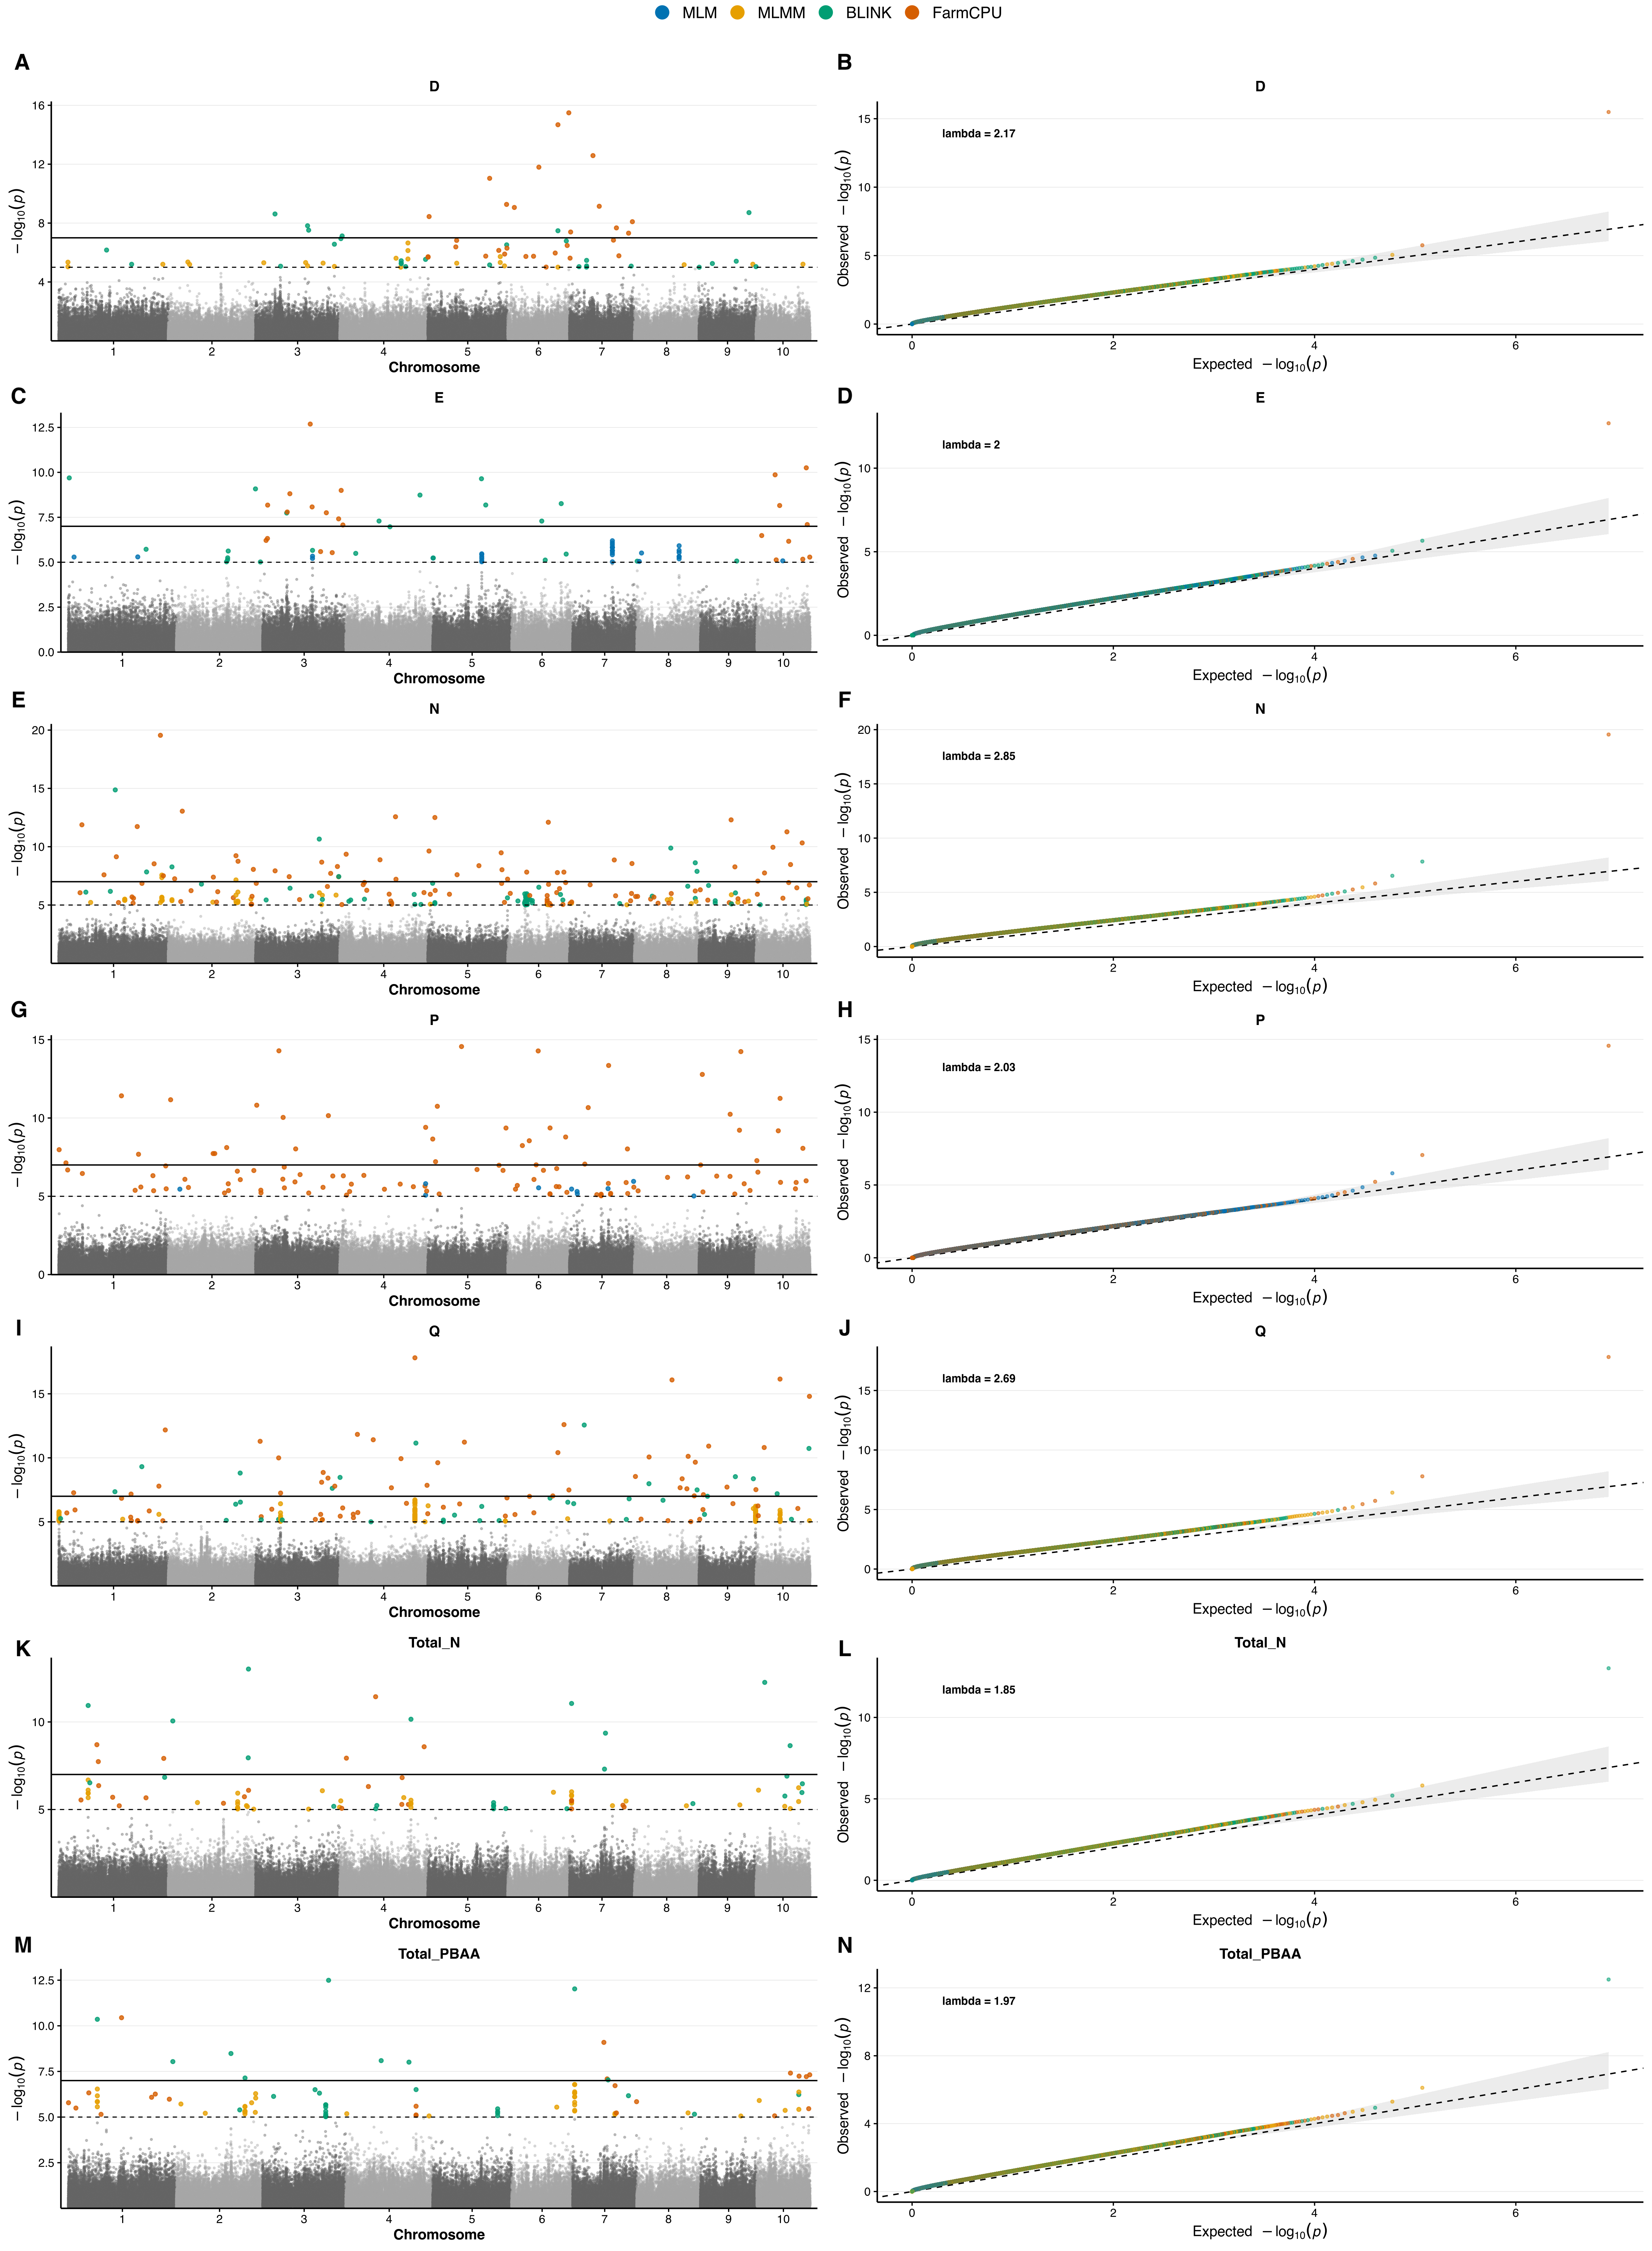
\includegraphics[width=\textwidth]{Figs/Supplementary/Supp_AminoAcid_Selected_Manhattan_QQ.png}
    \caption{Supplementary GWAS results for selected amino acid and nitrogen-related traits. For each trait, the Manhattan plot is shown on the left and the corresponding quantile--quantile plot on the right. Traits shown are D, E, N, P, Q, Total\_N, and Total\_PBAA. Colored points denote loci identified by the MLM, MLMM, BLINK, and FarmCPU models.}
    \label{fig:supp_amino_gwas}
\end{figure*}

\begin{figure*}[!htbp]
    \centering
    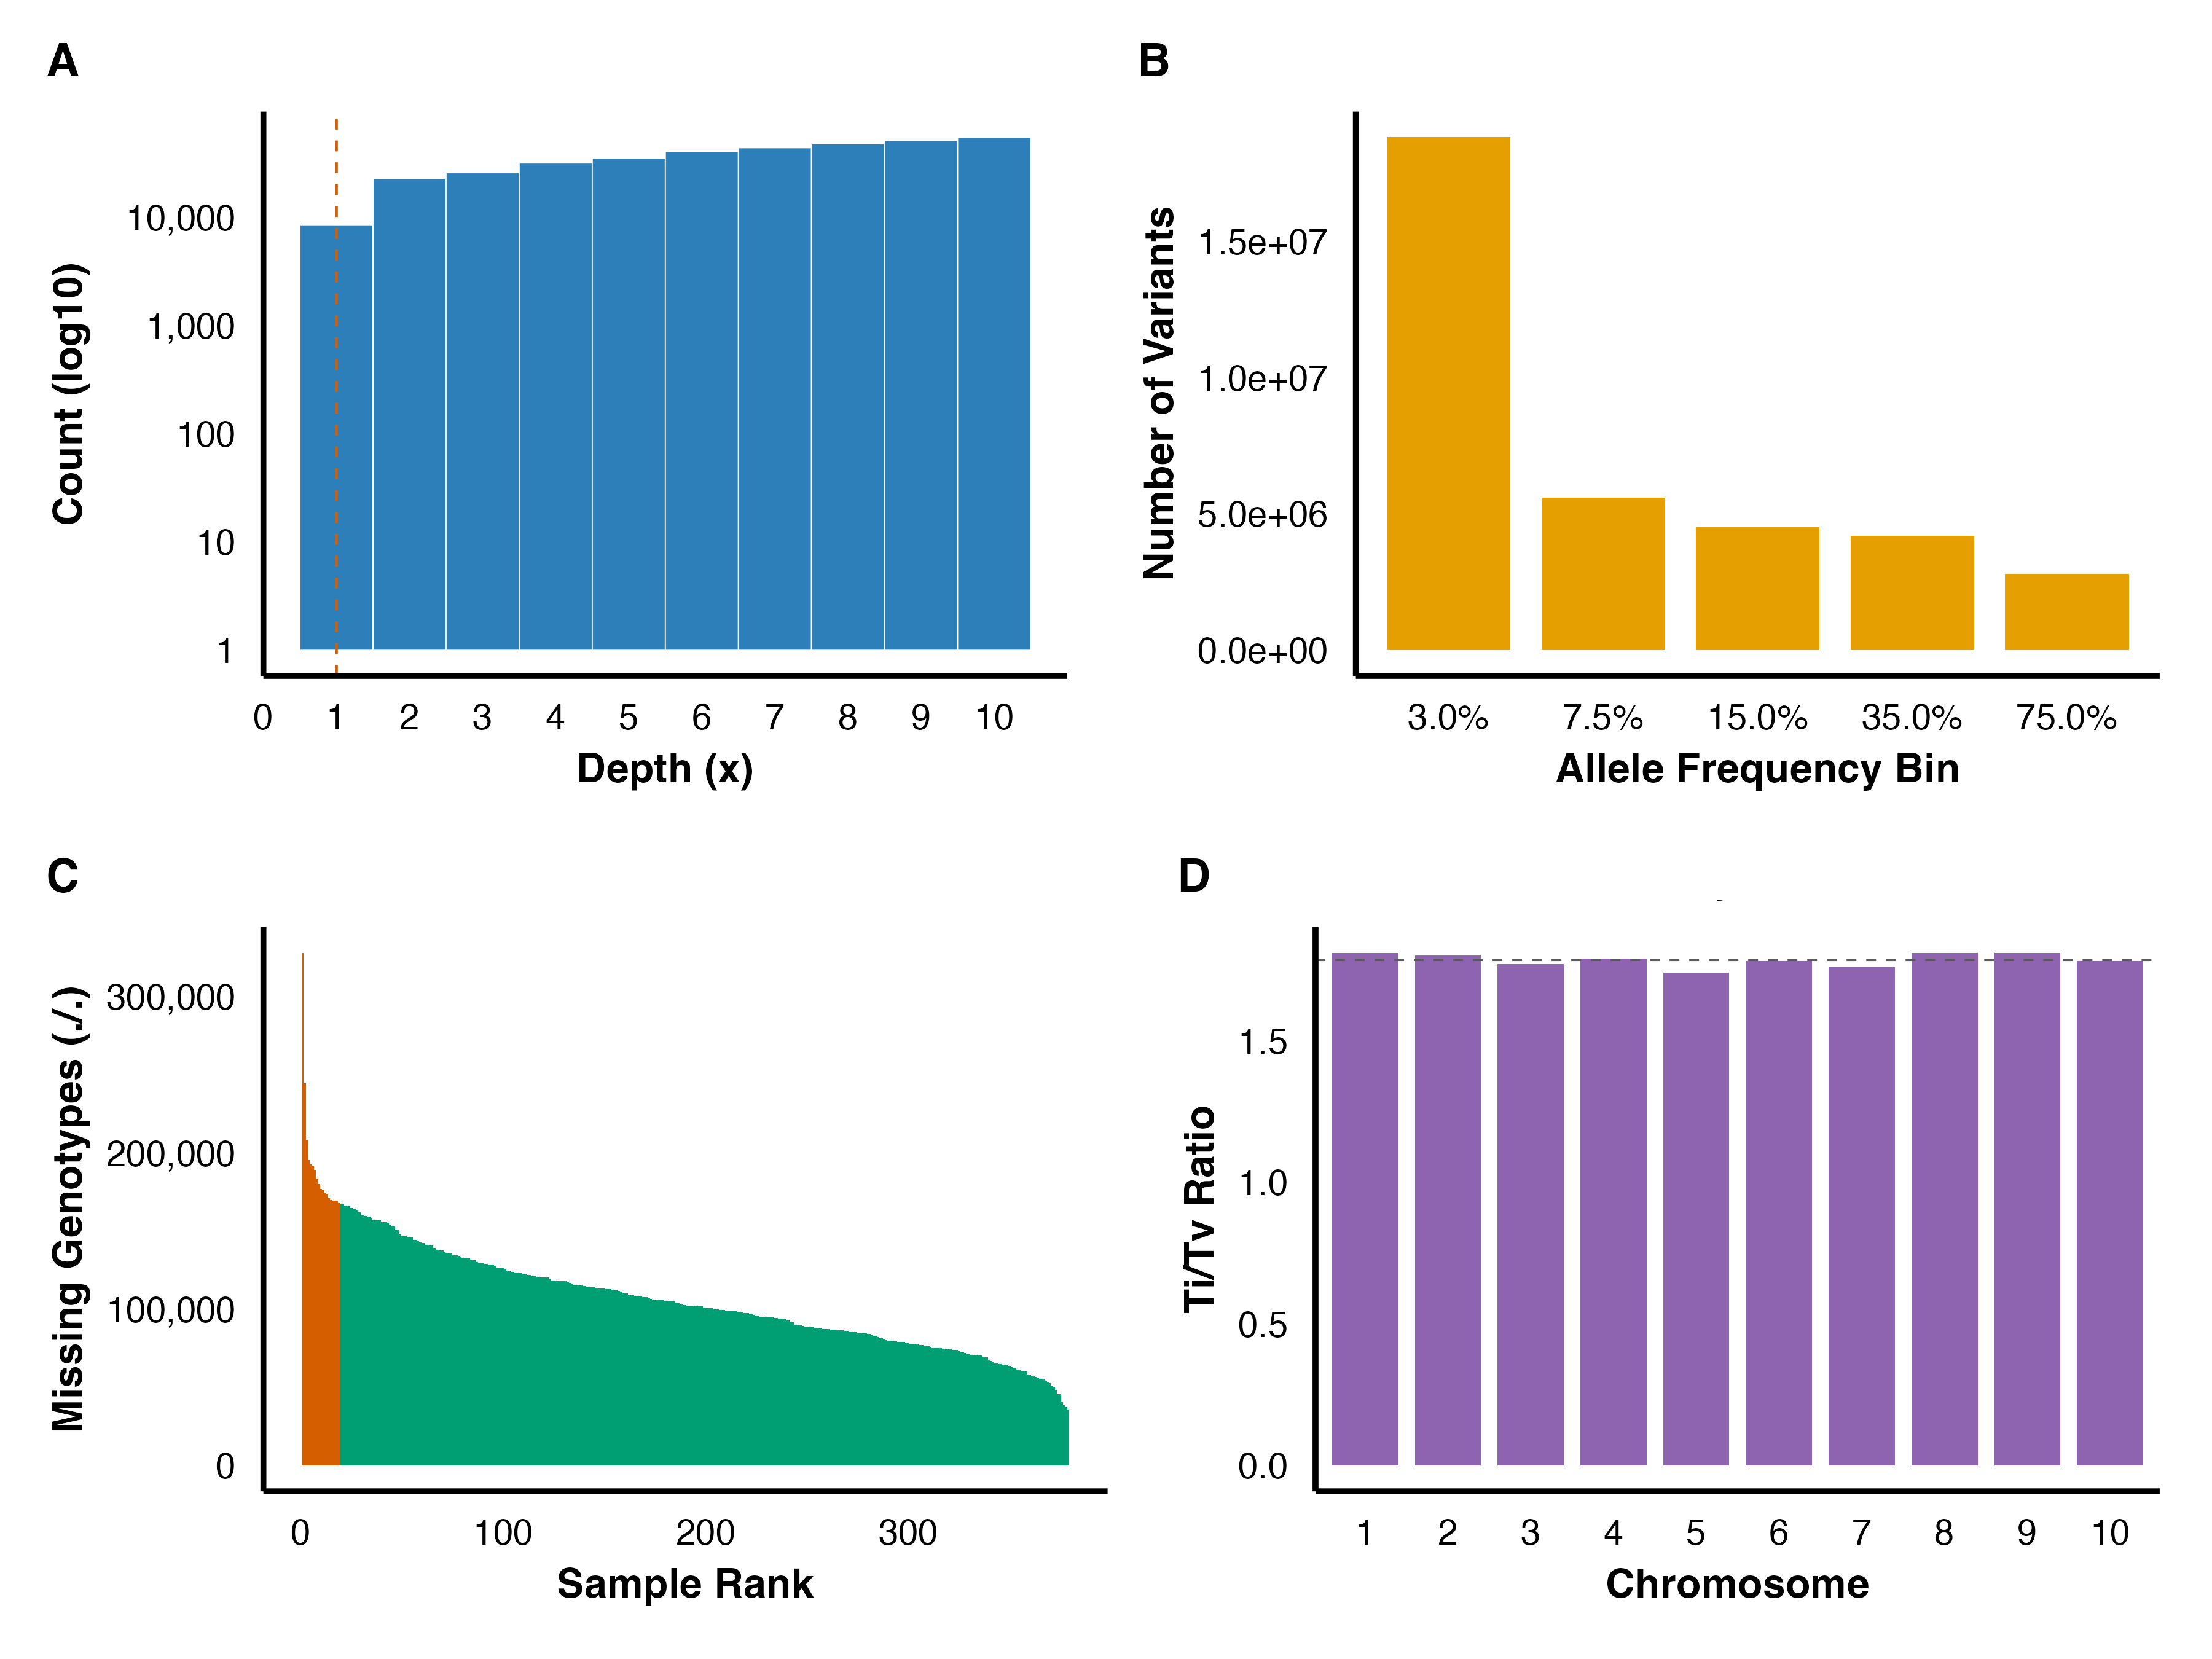
\includegraphics[width=\textwidth]{Figs/Supplementary/SuppFig_seq_statistics_variant_level.png}
    \caption{Supplementary variant-level quality summaries for the skim-sequencing data set. \textbf{A}, Variant depth distribution. \textbf{B}, Minor allele frequency spectrum. \textbf{C}, Missing genotypes per sample ranked across individuals. \textbf{D}, Transition/transversion ratio by chromosome.}
    \label{fig:supp_seq_variant}
\end{figure*}

\begin{figure*}[!htbp]
    \centering
    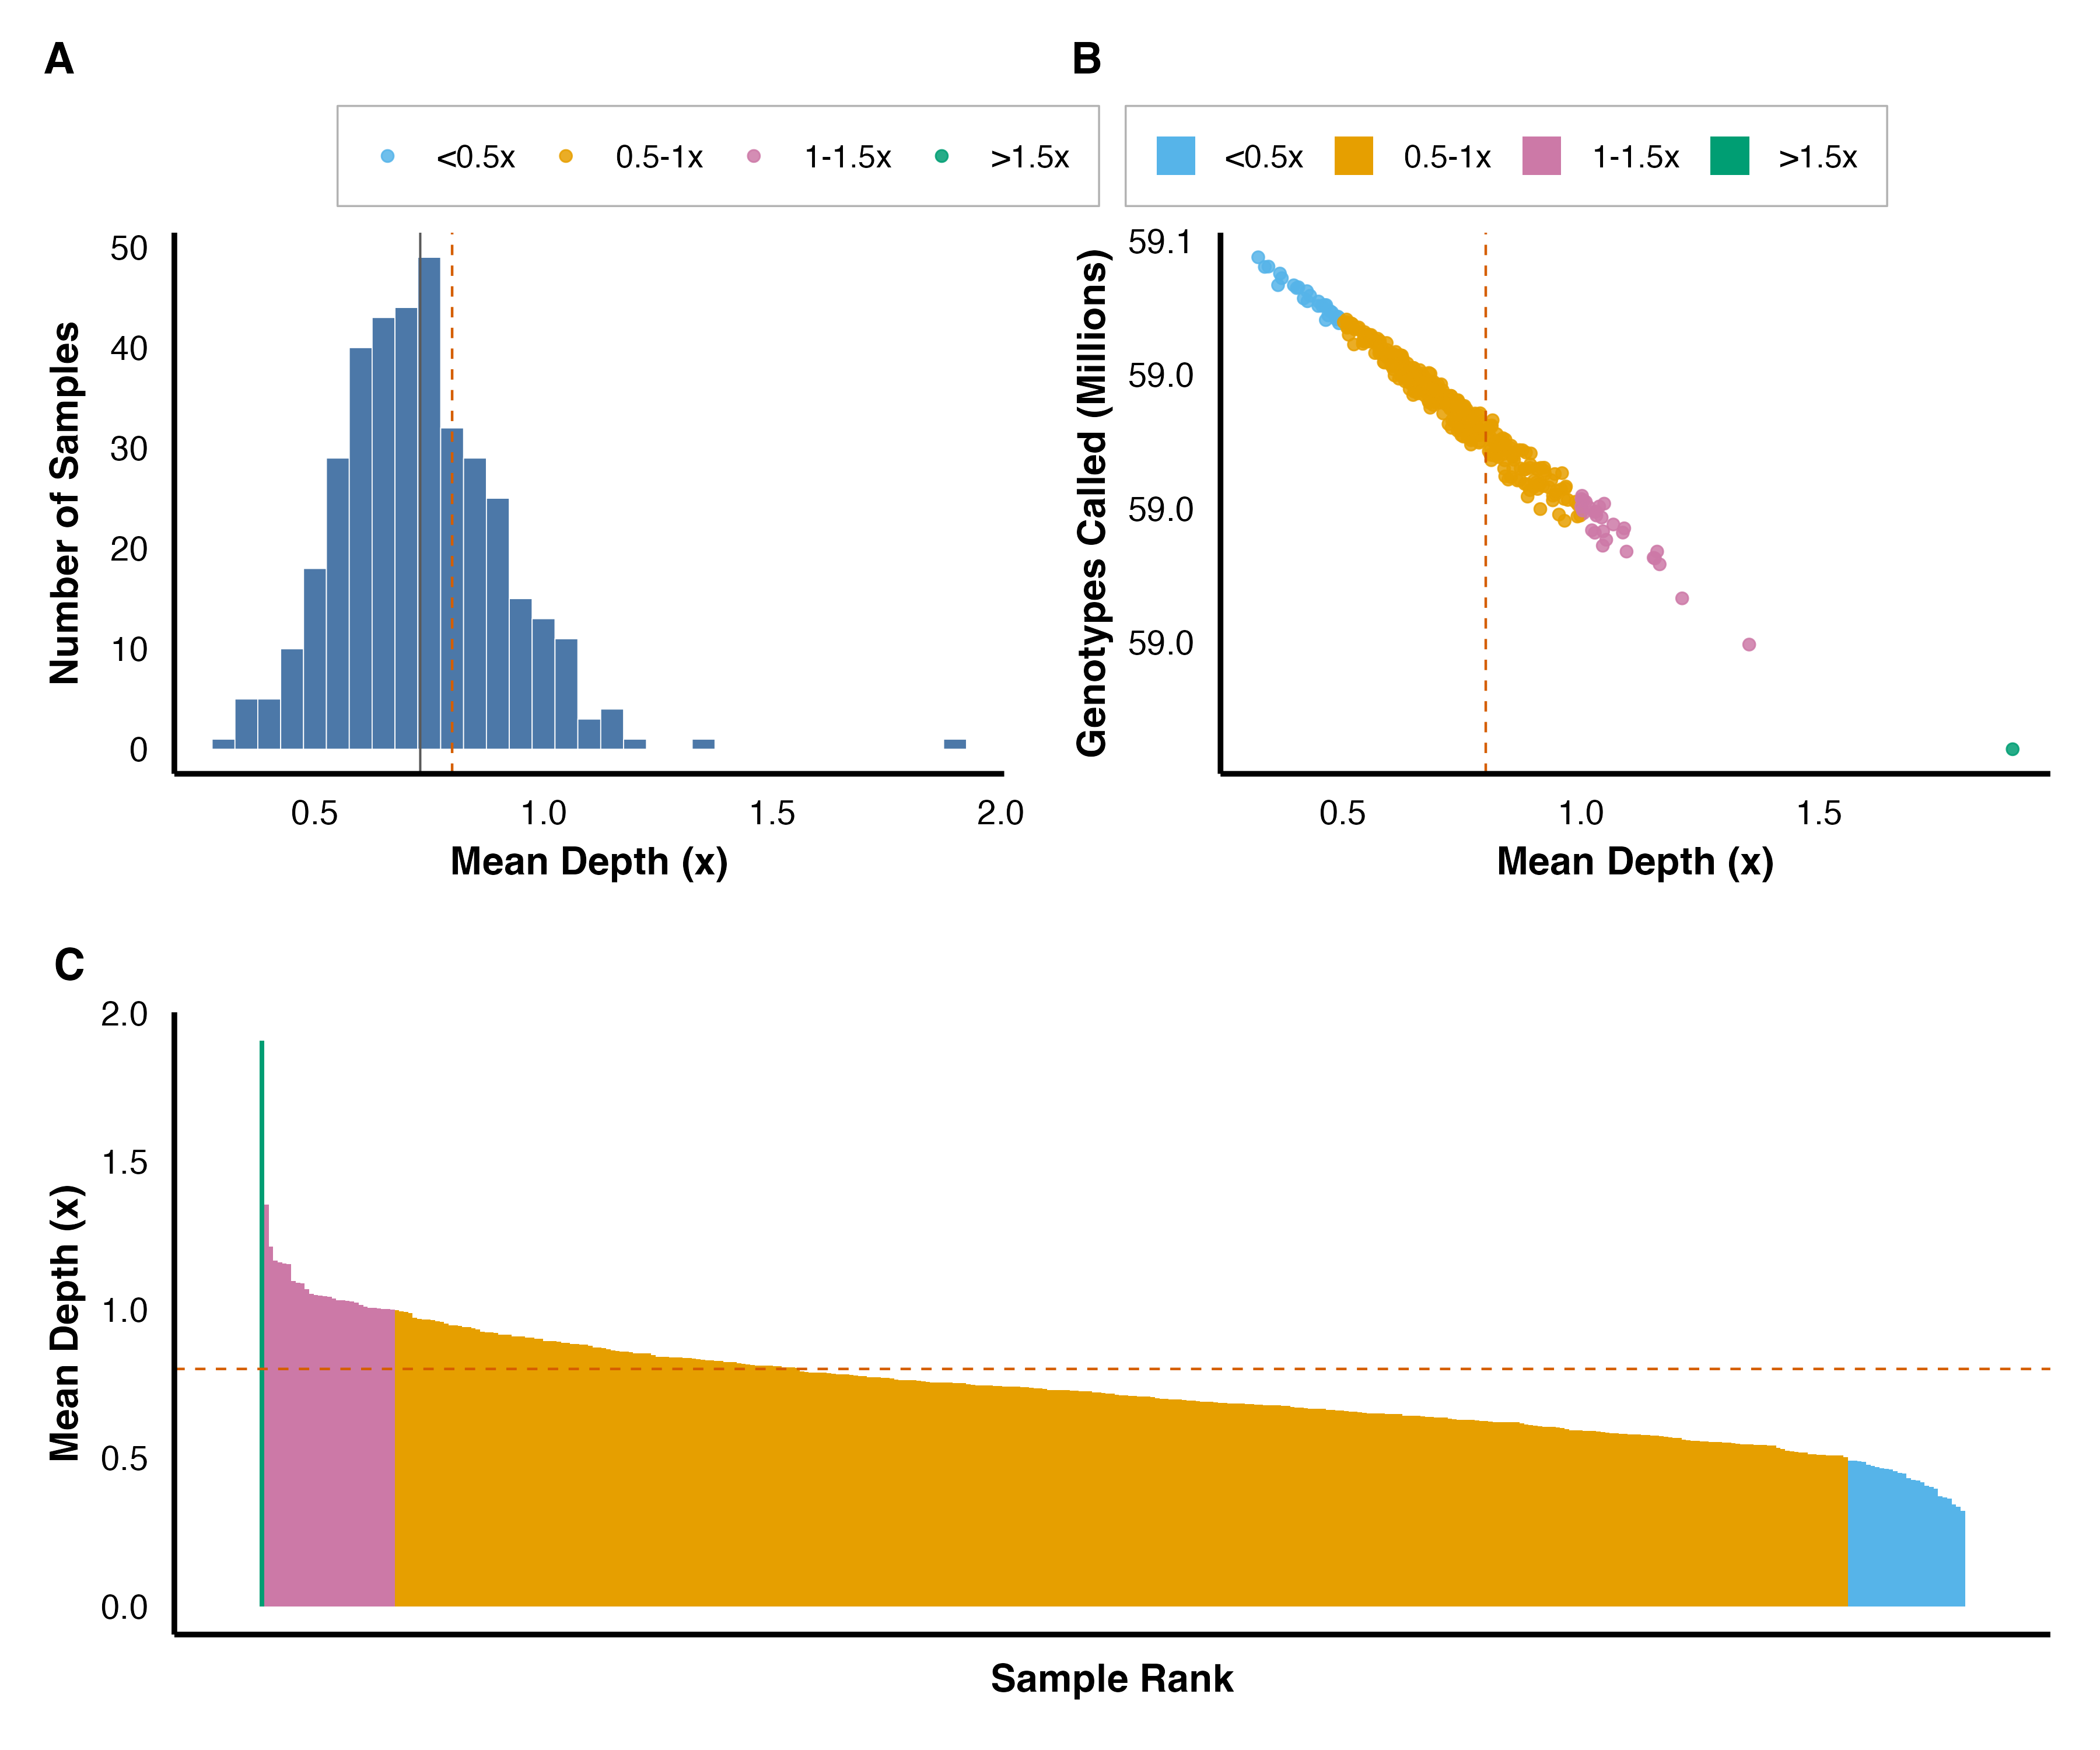
\includegraphics[width=\textwidth]{Figs/Supplementary/SuppFig_seq_statistics_sample_level.png}
    \caption{Supplementary sample-level quality summaries for the skim-sequencing data set. \textbf{A}, Distribution of mean sequencing depth across samples. \textbf{B}, Relationship between mean depth and the number of called genotypes per sample. \textbf{C}, Ranked sample depth across all sequenced individuals.}
    \label{fig:supp_seq_sample}
\end{figure*}

%%=============================================%%
%% For submissions to Nature Portfolio Journals %%
%% please use the heading ``Extended Data''.   %%
%%=============================================%%

%%=============================================================%%
%% Sample for another appendix section			       %%
%%=============================================================%%

%% \section{Example of another appendix section}\label{secA2}%
%% Appendices may be used for helpful, supporting or essential material that would otherwise 
%% clutter, break up or be distracting to the text. Appendices can consist of sections, figures, 
%% tables and equations etc.

\end{appendices}

%%===========================================================================================%%
%% If you are submitting to one of the Nature Portfolio journals, using the eJP submission   %%
%% system, please include the references within the manuscript file itself. You may do this  %%
%% by copying the reference list from your .bbl file, paste it into the main manuscript .tex %%
%% file, and delete the associated \verb+\bibliography+ commands.                            %%
%%===========================================================================================%%

\bibliography{sn-bibliography}% common bib file
%% if required, the content of .bbl file can be included here once bbl is generated
%%\input sn-article.bbl

\end{document}
